\documentclass[12pt]{report}
\usepackage[top=3cm, bottom=2.5cm, left=2cm, right=2.5cm]{geometry}
\usepackage{listings}
\usepackage{float}
\usepackage{subfig}
\usepackage{graphicx}
\usepackage{adjustbox}
\usepackage{ptext}
\usepackage[usenames,dvipsnames]{color,xcolor}
\usepackage{xepersian}
\settextfont[Scale=1]{XB Niloofar}
\definecolor{listinggray}{gray}{.98}
\lstset{language=Java,backgroundcolor=\color{listinggray},frameround=fttt,frame=trBL,basicstyle=\ttfamily,keywordstyle=\color{blue}\bfseries,numberstyle=\footnotesize,numbersep=10pt,numbers=left,captionpos=b,breaklines=true,showstringspaces=true}

\title{تمرین سری اول درس الگوریتم‌های معاملاتی}
\author{کورش تقی پور پاسدار}

\begin{document}
	\maketitle
\section{ورود و خروج از Position}

ما در ابتدا از استراتژی \lr{SMA} برای ورود به پوزیشن استفاده می‌کنیم. کد \lr{PineScript} این استراتژی، همان کد موجود برروی سابت \lr{TradingView} می‌باشد.
\begin{latin}
\lstinputlisting{strategy_1.txt}
\label{code1}
\end{latin}
در این کد، ابتدا میانگین ساده \lr{Simple Moving Average} برای ۱۲ و ۲۶ کندل حساب می‌شود. سپس از روی رخداد کراس رو به بالا یا پایین، به ترتیب پوزیشن \lr{long} یا \lr{short} باز می‌شود.کراس رو به بالا نشان‌دهنده روند صعودی‌تر بازار در بازه اخیر نسبت به بازه‌های قدیمی‌تر است و کراس رو به پایین نیز عکس این موضوع را نشان می‌دهد. همچنین در هنگام باز‌کردن پوزیشن \lr{long} یا \lr{short}، درصورتیکه پوزیشن مخالف باقی‌ مانده باشد، تابع \lr{strategy.entry} آن را به طور خودکار هندل می‌کند.
\begin{figure}[h!]
	\centering
	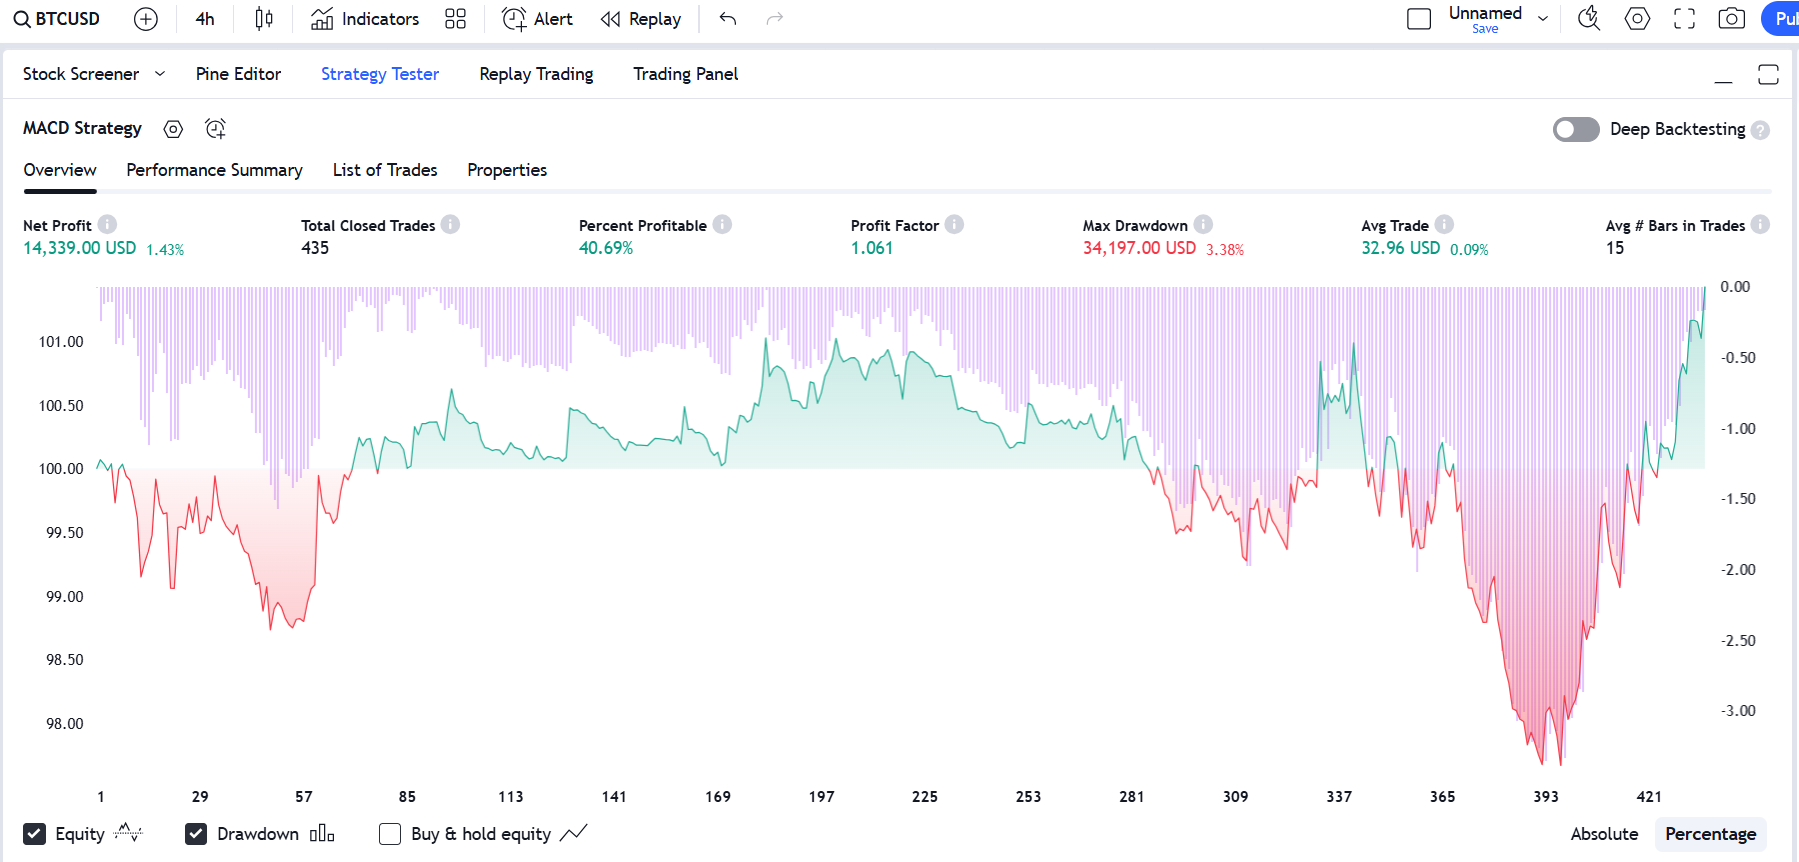
\includegraphics[scale=0.3]{pic_1.png}
	\caption{عملکرد استراتژی \lr{SMA} برروی بیتکوین به دلار}
	\label{p1}
\end{figure}
\newline
همانگونه که در تصویر \ref{p1} مشاهده می‌شود، این استراتژی عملکرد نسبتا خوبی برروی یک بازه‌ای از زمان دارد.
\begin{figure}[H]
	\centering
	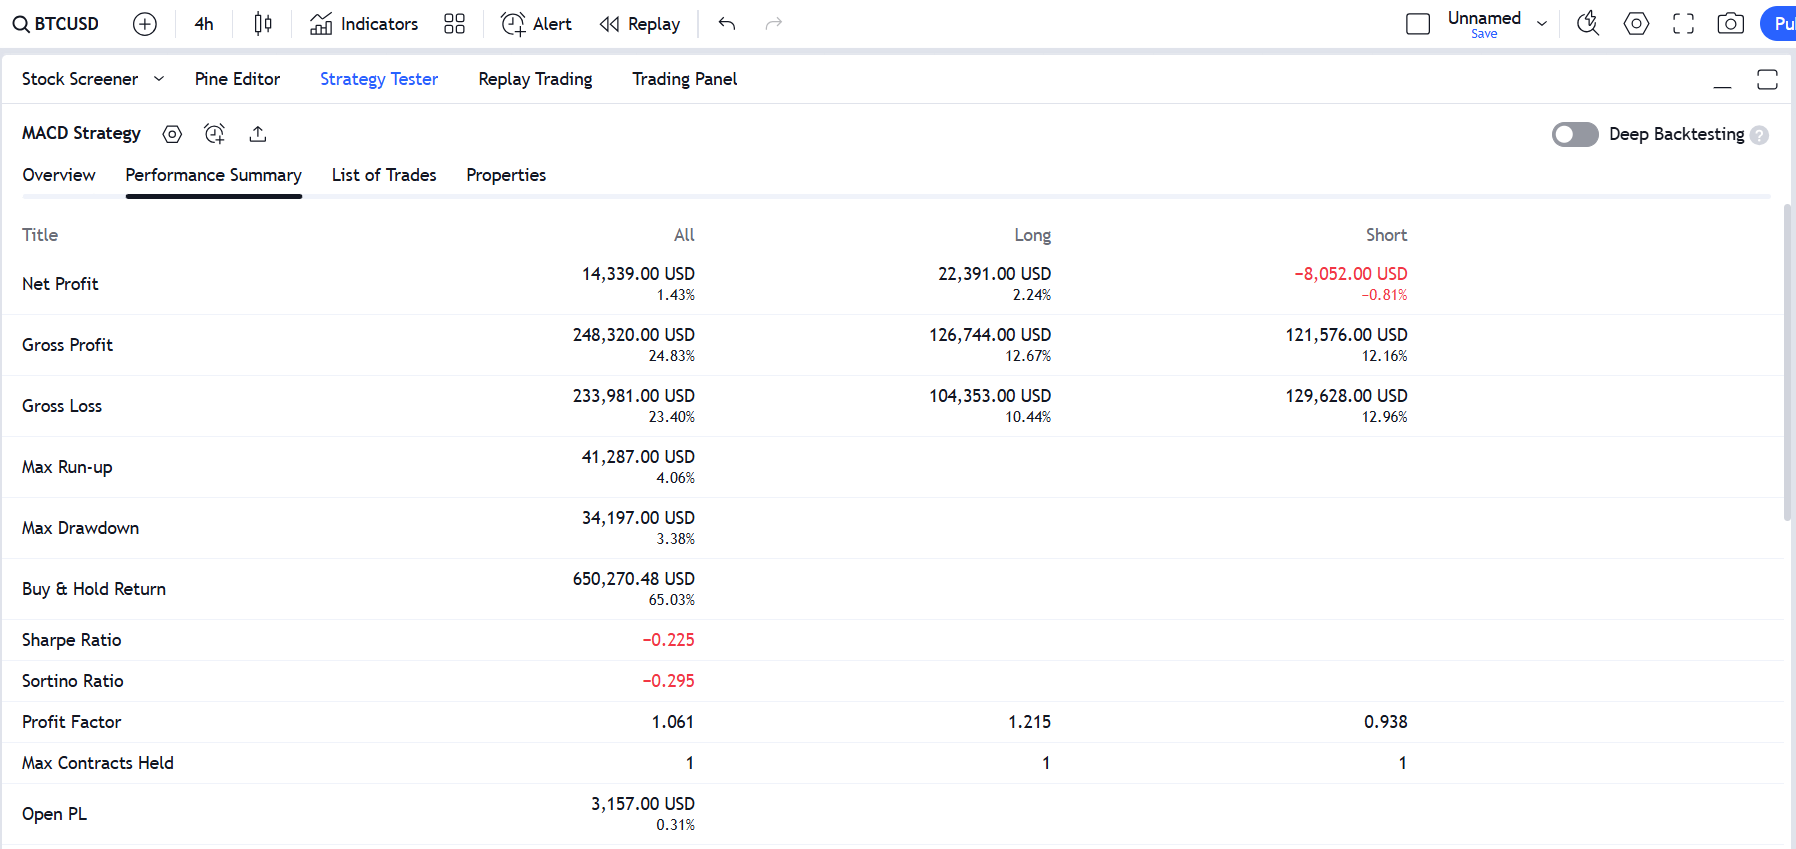
\includegraphics[scale=0.3]{pic_2.png}
	\caption{سود و زیان استراتژی در پوزیشن‌های \lr{short} و \lr{long} و سود و زیان کلی}
	\label{p2}
\end{figure}
طبق تصویر \ref{p2} ، این استراتژی برروی پوزیشن‌های \lr{short} عملکرد زیان‌ده نشان داده است ولی برروی پوزیشن‌های \lr{long} سودده بوده است.
\newline
حال عملکرد استراتژی \lr{EMA} را برروی همان داده‌ها بررسی می‌کنیم. کد \lr{PineScript} آن مشابه استراتژی قبلی بوده، با این تفاوت که بجای تابع \lr{ta.sma} از تابع \lr{ta.ema} استفاده شده است. برای عدم تکرار، اصل کد آورده نمی‌شود.
\begin{figure}[H]
	\centering
	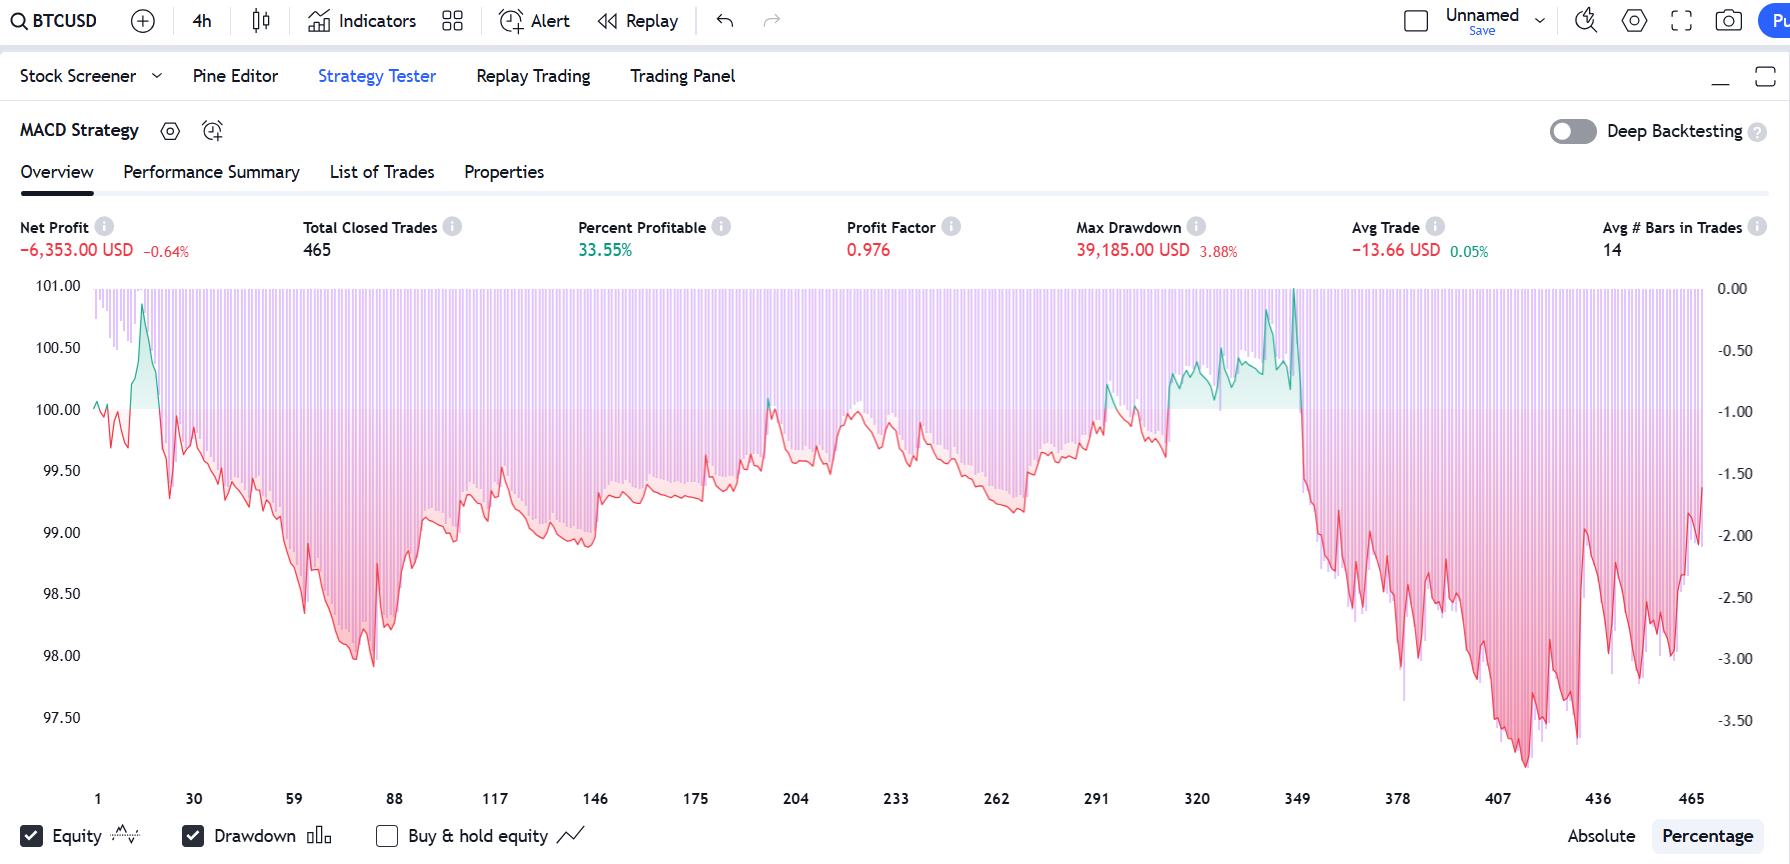
\includegraphics[scale=0.3]{pic_3.png}
	\caption{عملکرد استراتژی \lr{EMA} برروی بیتکوین به دلار}
	\label{p3}
\end{figure}
همانگونه که در تصویر \ref{p3} نشان داده می‌شود، این استراتژی عملکرد زیان ده داشته است و به ندرت بازه‌های سودده به چشم می‌خورد.
\begin{figure}[H]
	\centering
	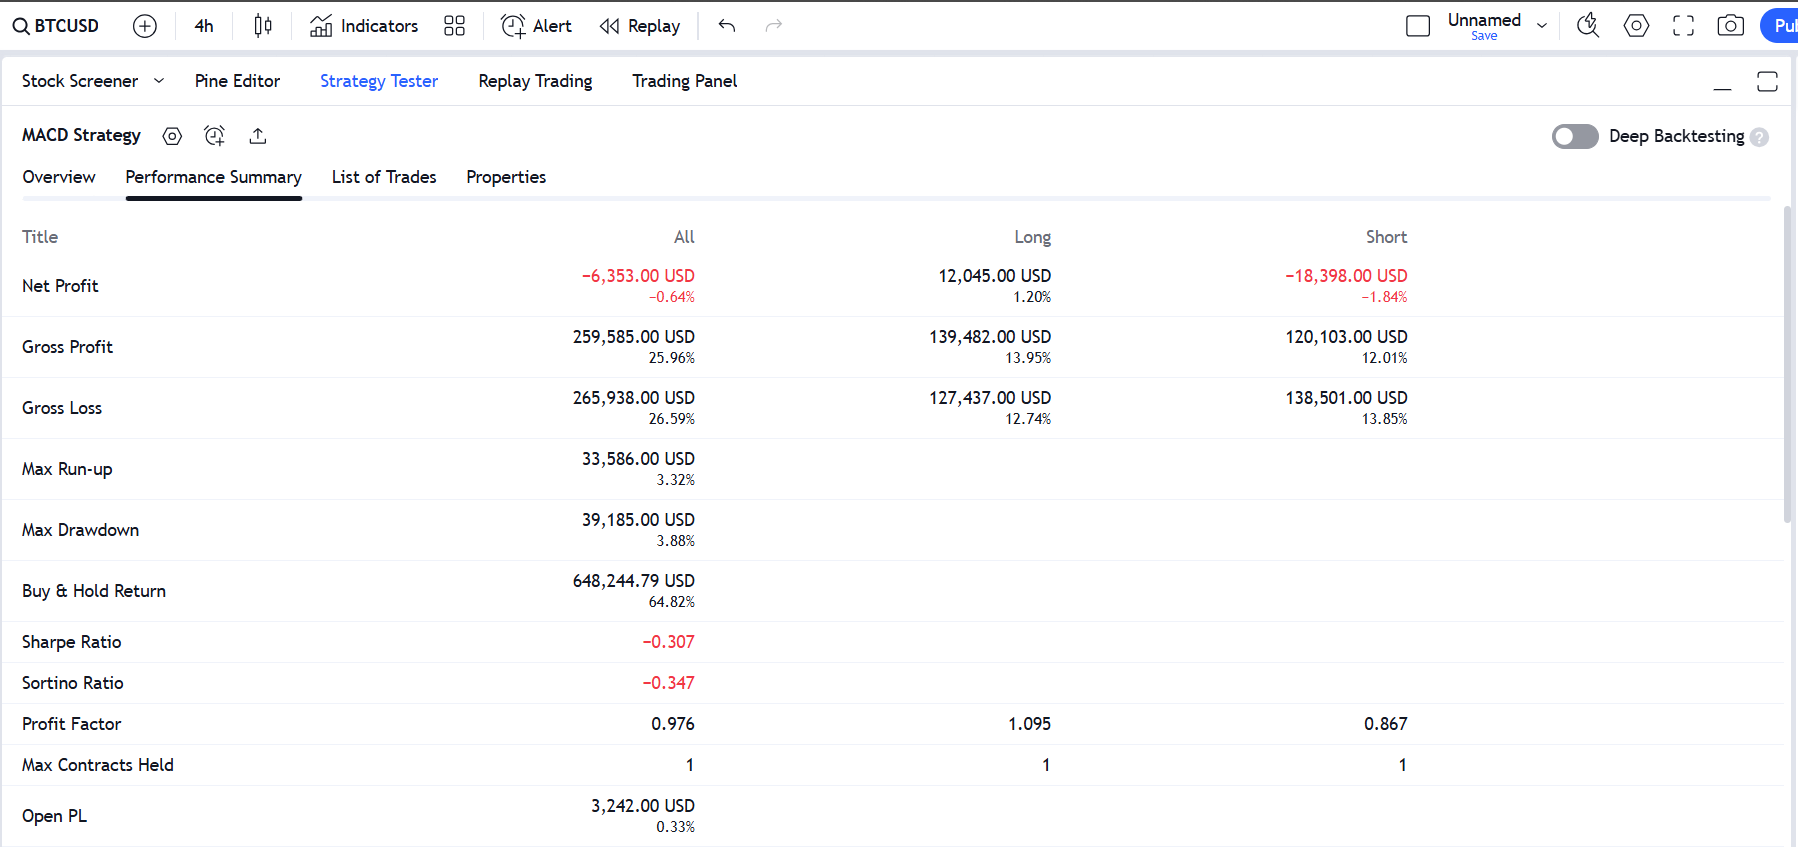
\includegraphics[scale=0.3]{pic_4.png}
	\caption{سود و زیان استراتژی \lr{EMA} در پوزیشن‌های \lr{short} و \lr{long}}
	\label{p4}
\end{figure}
مشابه استراتژی \lr{SMA}، این استراتژی نیز برروی پوزیشن‌های \lr{short}
عملکرد زیان‌ده داشته و برروی پوزیشن‌های \lr{long} عملکرد سودده داشته است ولی درمجموع عملکرد زیان‌ده داشته است.
\newline
با مقایسه متریک‌های این دو استراتژی، مانند \lr{Sharpe Ratio}، به این نتیجه می‌رسیم که استراتژی \lr{EMA} ریسک بیشتری نسبت به استراتژی \lr{SMA} متحمل می‌شود و در نتیجه نتیجه بدتری در بر دارد.
\section{استفاده از \lr{RSI} برای تایید قوت سیگنال}
حال در این بخش، از \lr{ًRSI} برای تشخیص بهتر سیگنال استفاده می‌کنیم. در کد زیر، کد \lr{PineScript} مربوط به استراتژی \lr{RSI} موجود در سایت \lr{TradingView} آورده شده است.
\begin{latin}
	\lstinputlisting{rsi_strategy.txt}
\end{latin}
در کد بالا، در ابتدا مقدار \lr{RSI} تعیین می‌شود. \lr{RSI} درواقع سرعت و بزرگی تغییرات قیمت یک سهام را اندازه‌گیری می‌کند و در ادامه با استفاده از مقادیر \lr{OverBought} , \lr{OverSold} حد بازکردن پوزیشن \lr{long} یا \lr{short} را تعیین می‌کند. این کد به ما در ارتقای کد \ref{code1} کمک می‌کند.
\newline
\begin{latin}
	\lstinputlisting{macd_rsi_sma.txt}
	\label{code2}
\end{latin}
کد بالا، کد بهبودیافته \ref{code1} با استفاده از استراتژی \lr{RSI} می‌باشد. در این کد، ما بازکردن پوزیشن خرید یا فروش را صرفا منوط به رخداد \lr{cross} قرار نداده‌ایم،‌ بلکه تازمانیکه به سقف خرید و فروش نرسیده‌ایم، به خرید و فروش سهام ادامه می‌دهد.
\begin{figure}[H]
	\centering
	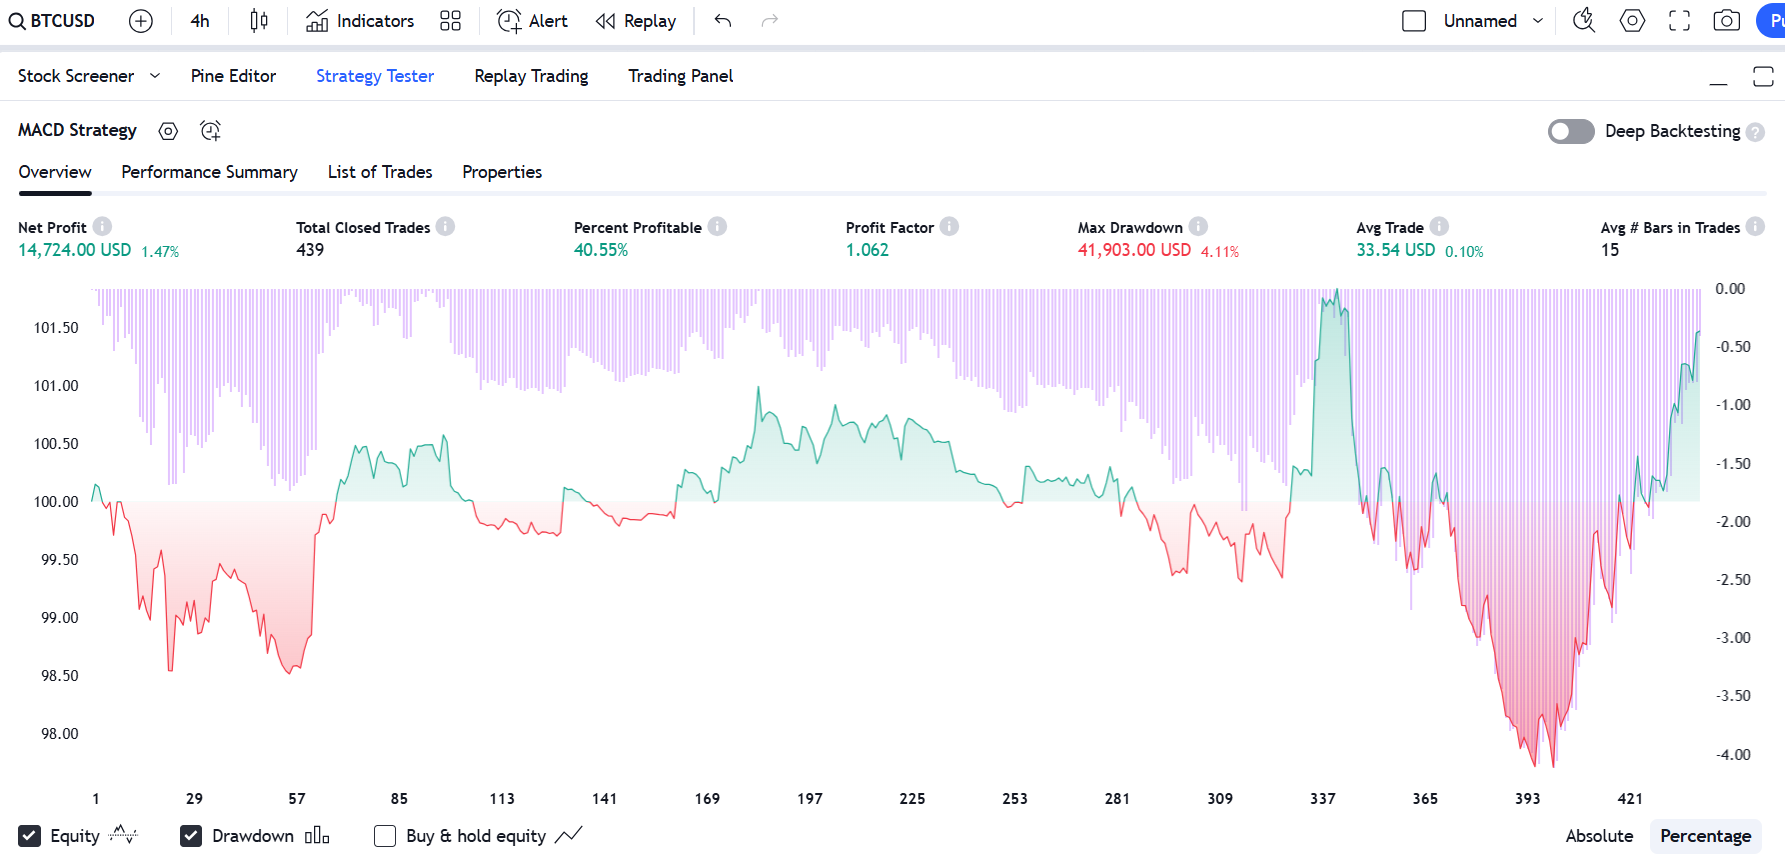
\includegraphics[scale=0.3]{pic_5.png}
	\caption{سود و زیان ترکیب استراتژی‌های \lr{SMA} و \lr{RSI}}
	\label{p5}
\end{figure}
همانگونه که در تصویر \ref{p5} مشاهده می‌شود، ما شاهد افزایش سود به میزان 325 دلار هستیم. هرچند در تصویر \ref{p6} نشان داده می‌شود مقدار سود و زیان چندان تغییری نکرده است.
\begin{figure}[H]
	\centering
	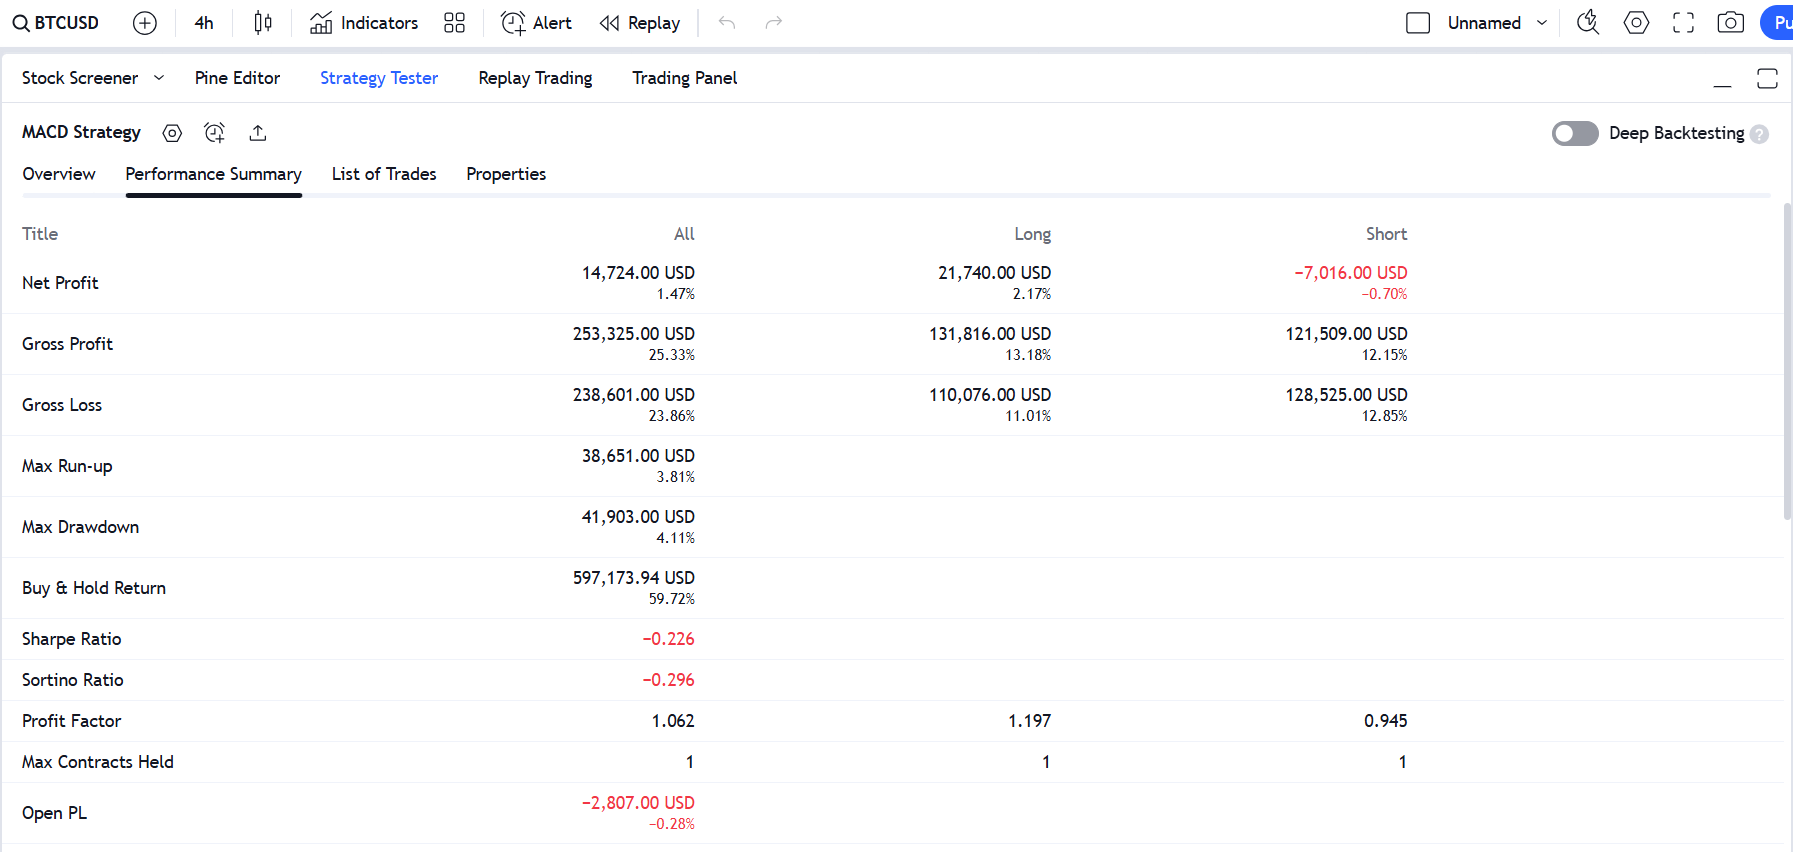
\includegraphics[scale=0.3]{pic_6.png}
	\caption{سود و زیان ترکیب استراتژی \lr{SMA} و \lr{RSI} در پوزیشن‌های \lr{short} و \lr{long}}
	\label{p6}
\end{figure}
حال استراتژی \lr{EMA} را با استراتژی \lr{RSI} ترکیب می‌کنیم. کد این استراتژی مشابه کد \ref{code2} می‌باشد با این تفاوت که بجای تابع \lr{ta.sma} از تابع \lr{ta.ema} استفاده شده است.
\begin{figure}[H]
	\centering
	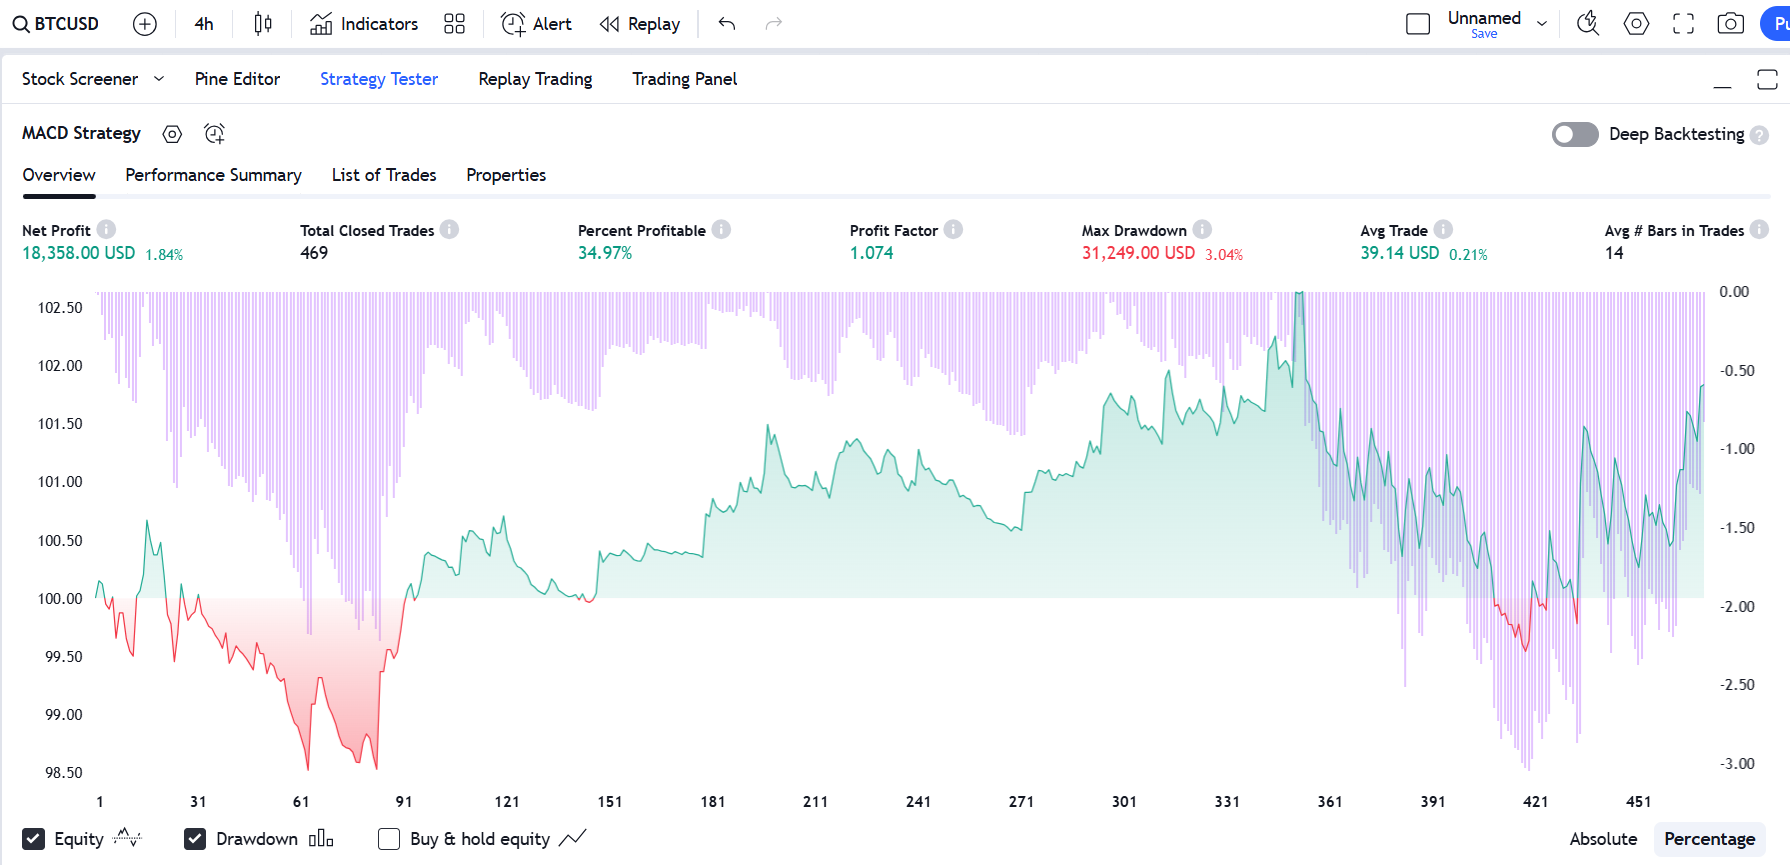
\includegraphics[scale=0.3]{pic_7.png}
	\caption{عملکرد ترکیب استراتژی‌های \lr{EMA} و \lr{RSI} برروی بیتکوین به دلار}
	\label{p7}
\end{figure}
تصویر \ref{p7} نشان می‌دهد برخلاف ترکیب دو استراتژی \lr{SMA} و \lr{RSI} که تاثیر چندانی بر عملکرد نداشت، ترکیب این دو استراتژی افزایش چشمگیری به ارمغان داشته و سوددهی را از \lr{-6353 USD} به \lr{18358 USD} رسانده است.
\begin{figure}[H]
	\centering
	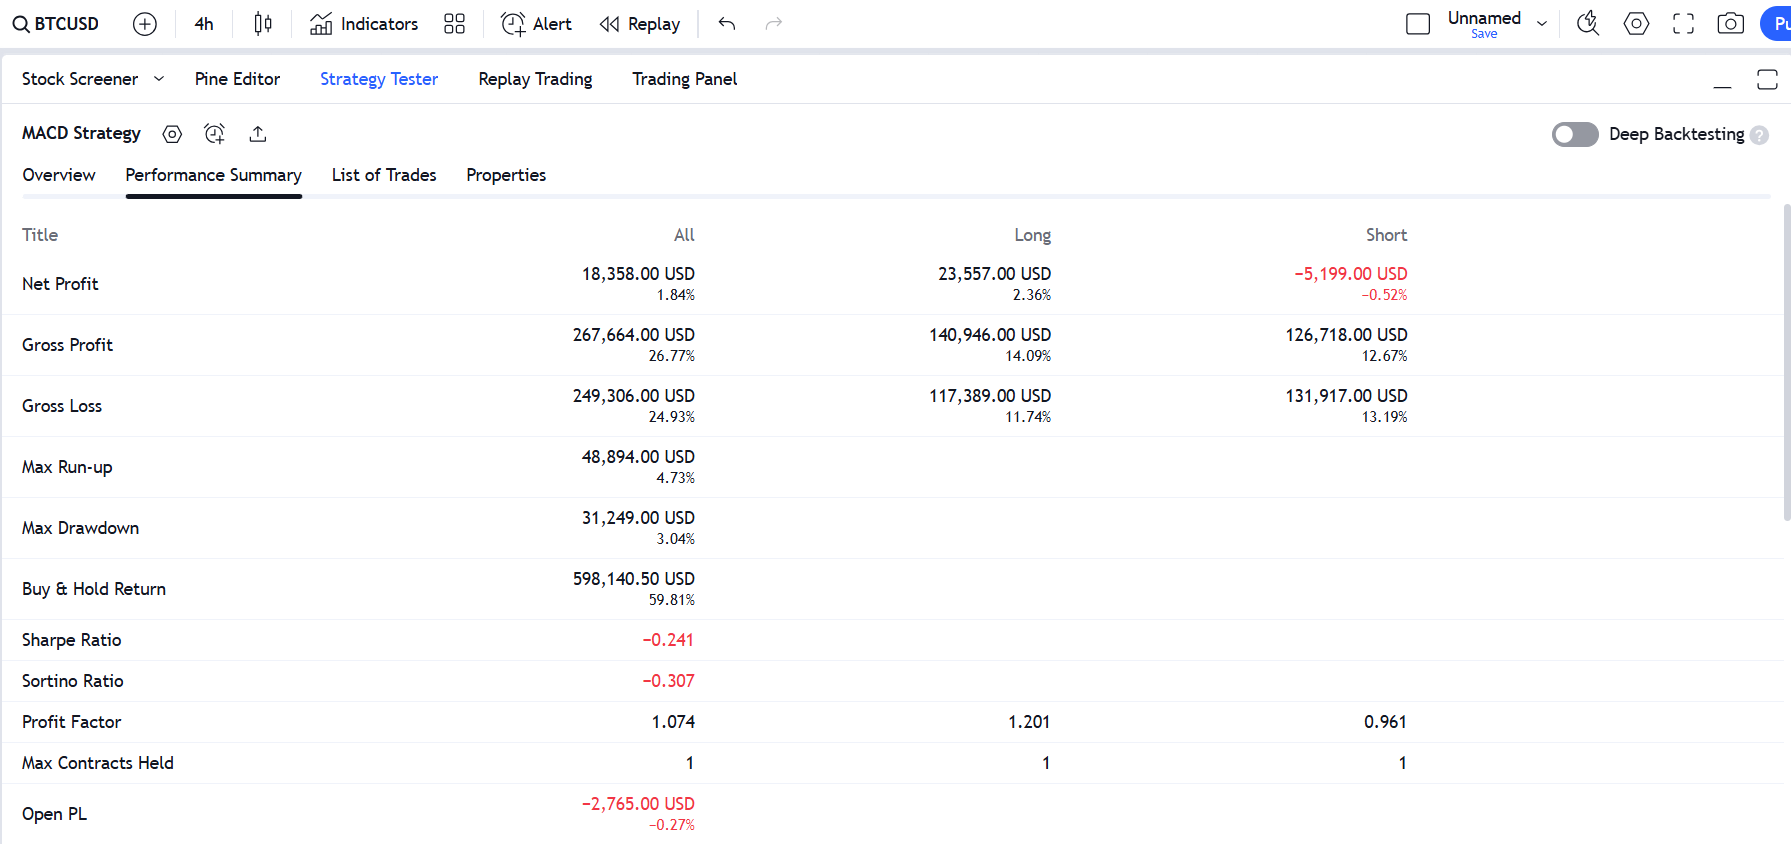
\includegraphics[scale=0.3]{pic_8.png}
	\caption{سود و زیان ترکیب استراتژی \lr{EMA} و \lr{RSI}}
	\label{p8}
\end{figure}
همچنین در تصویر \ref{p8} شاهد هستیم که میزان \lr{Sharpe Ratio} از \lr{-0.307} به \lr{-0.241} رسیده است که نشان‌دهنده کاهش ریسک این استراتژی می‌باشد.
\newpage
\section{تست استراتژی حاصل برروی سایر رمزارزها}
تست استراتژی برروی رمزارز \lr{ETH}
\begin{figure}[H]
	\centering
\subfloat[
عملکرد ترکیب استراتژی‌های \lr{EMA} و \lr{RSI} برروی رمزارز \lr{ETH}
]{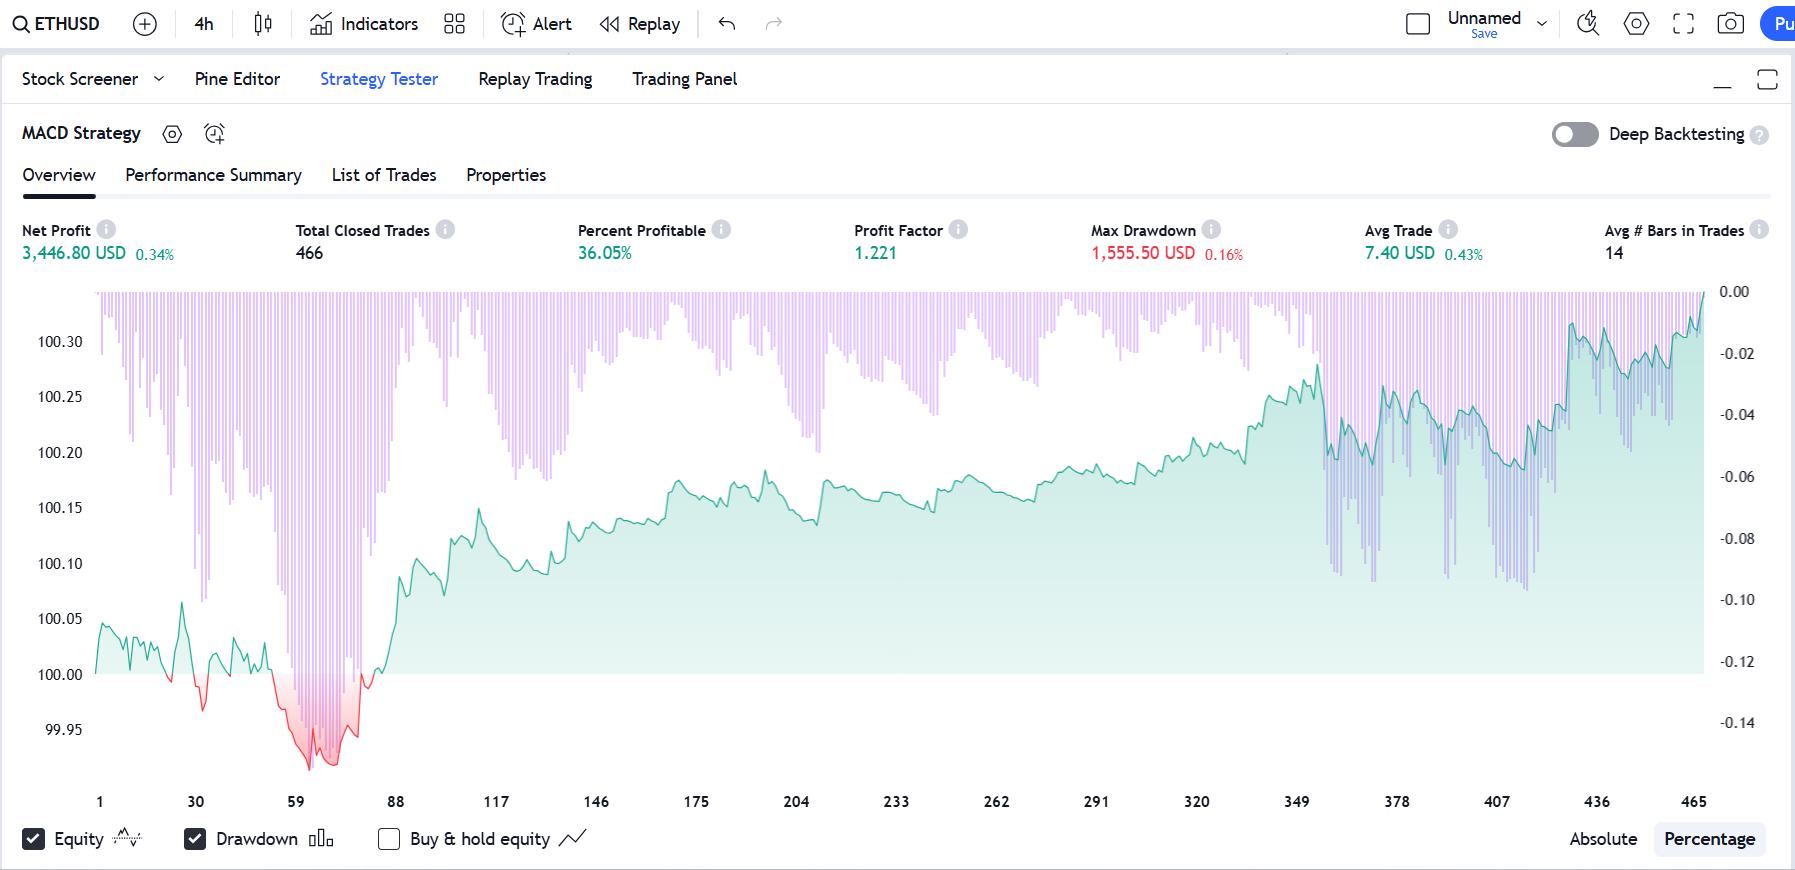
\includegraphics[scale=0.15]{pic_9.png}\label{p9}}
\quad \quad
\subfloat[
سود و زیان ترکیب استراتژی \lr{EMA} و \lr{RSI}
]{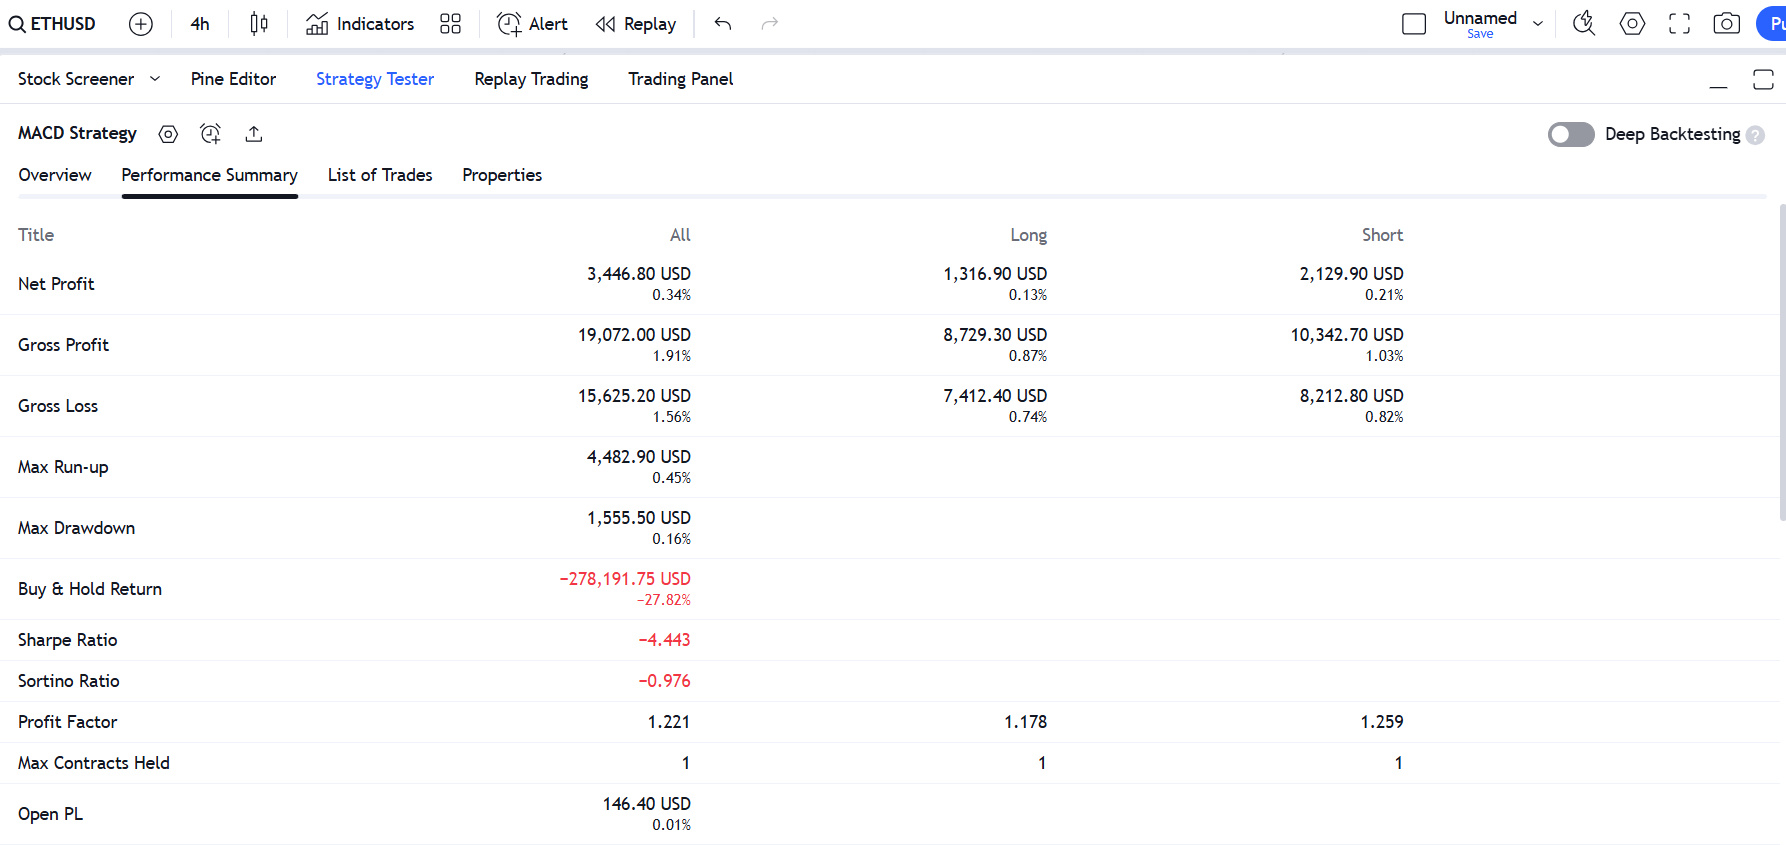
\includegraphics[scale=0.15]{pic_10.png}\label{p10}}
\end{figure}
تست استراتژی برروی رمزارز \lr{SOLANA}
\begin{figure}[H]
	\centering
\subfloat[
عملکرد ترکیب استراتژی‌های \lr{EMA} و \lr{RSI} برروی رمزارز \lr{SOLANA}
]{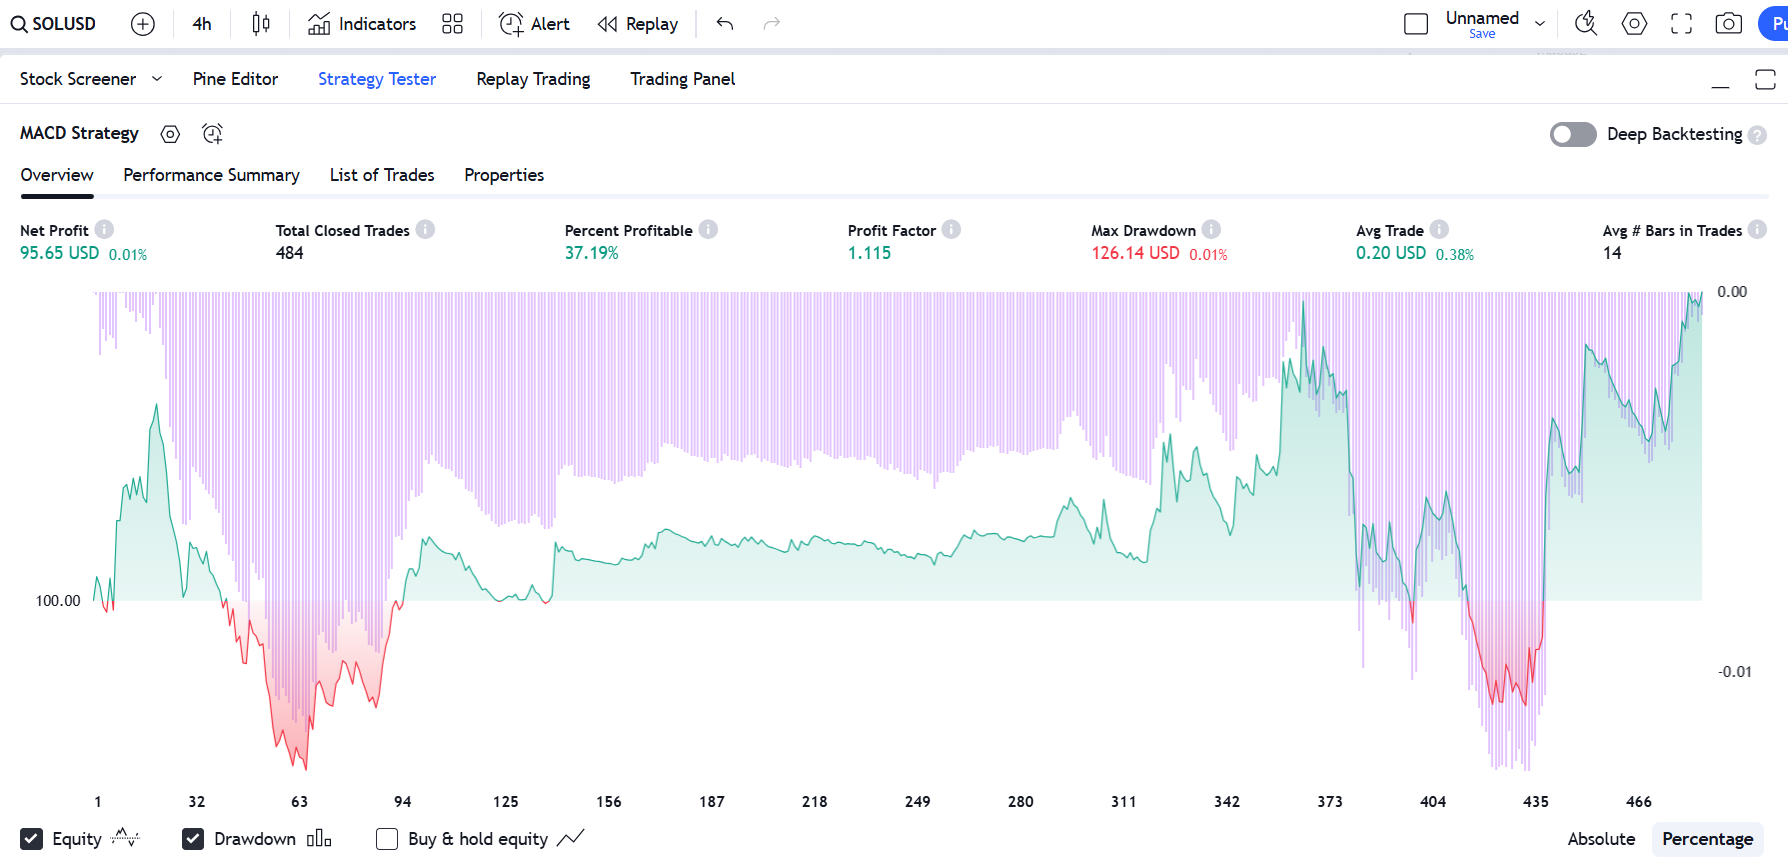
\includegraphics[scale=0.15]{pic_11.png}\label{p11}}
\quad \quad
\subfloat[
سود و زیان ترکیب استراتژی \lr{EMA} و \lr{RSI}
]{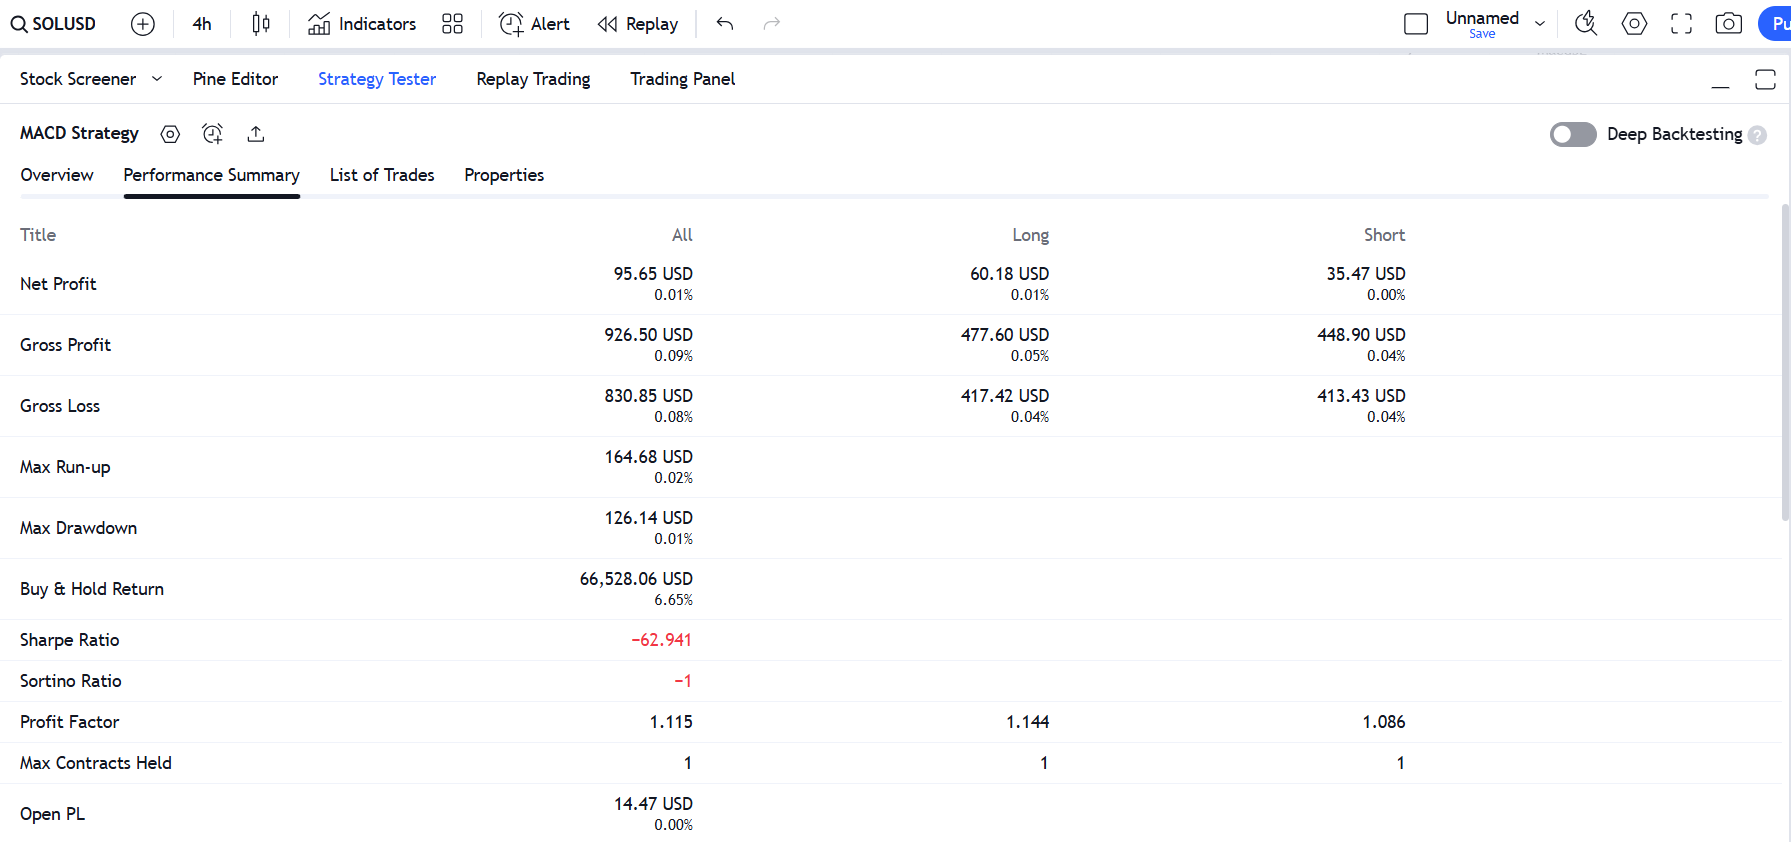
\includegraphics[scale=0.15]{pic_12.png}\label{p12}}
\end{figure}
تست استراتژی برروی رمزارز \lr{BNB}
\begin{figure}[H]
	\centering
	\subfloat[
	عملکرد ترکیب استراتژی‌های \lr{EMA} و \lr{RSI} برروی رمزارز \lr{BNB}
	]{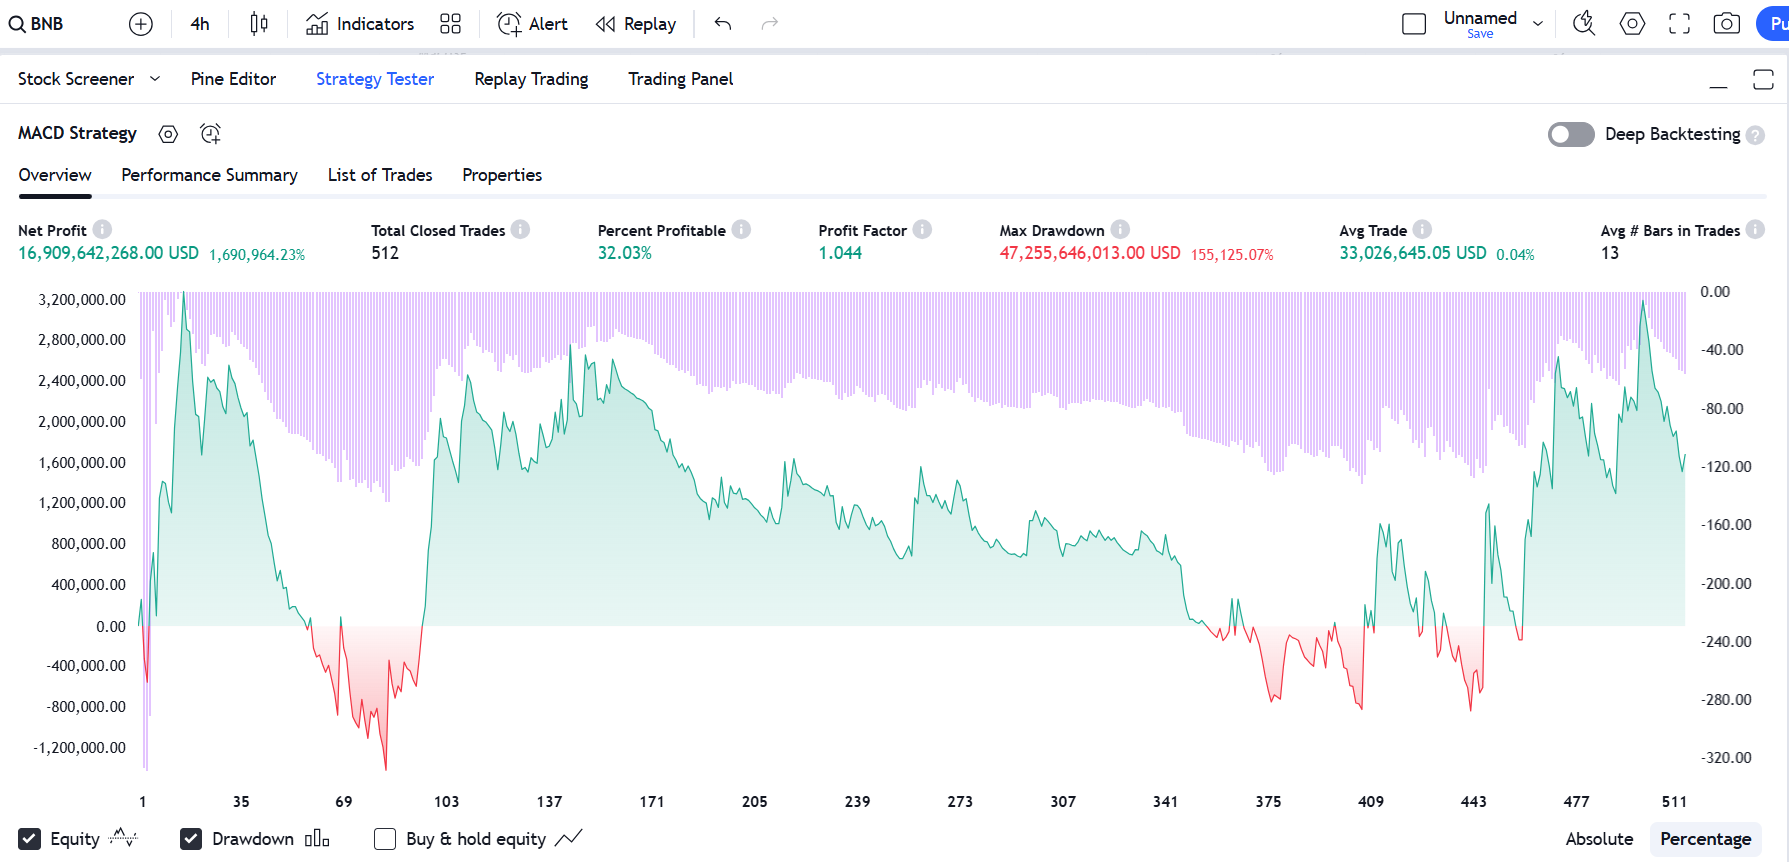
\includegraphics[scale=0.15]{pic_13.png}\label{p13}}
	\quad \quad
	\subfloat[
	سود و زیان ترکیب استراتژی \lr{EMA} و \lr{RSI}
	]{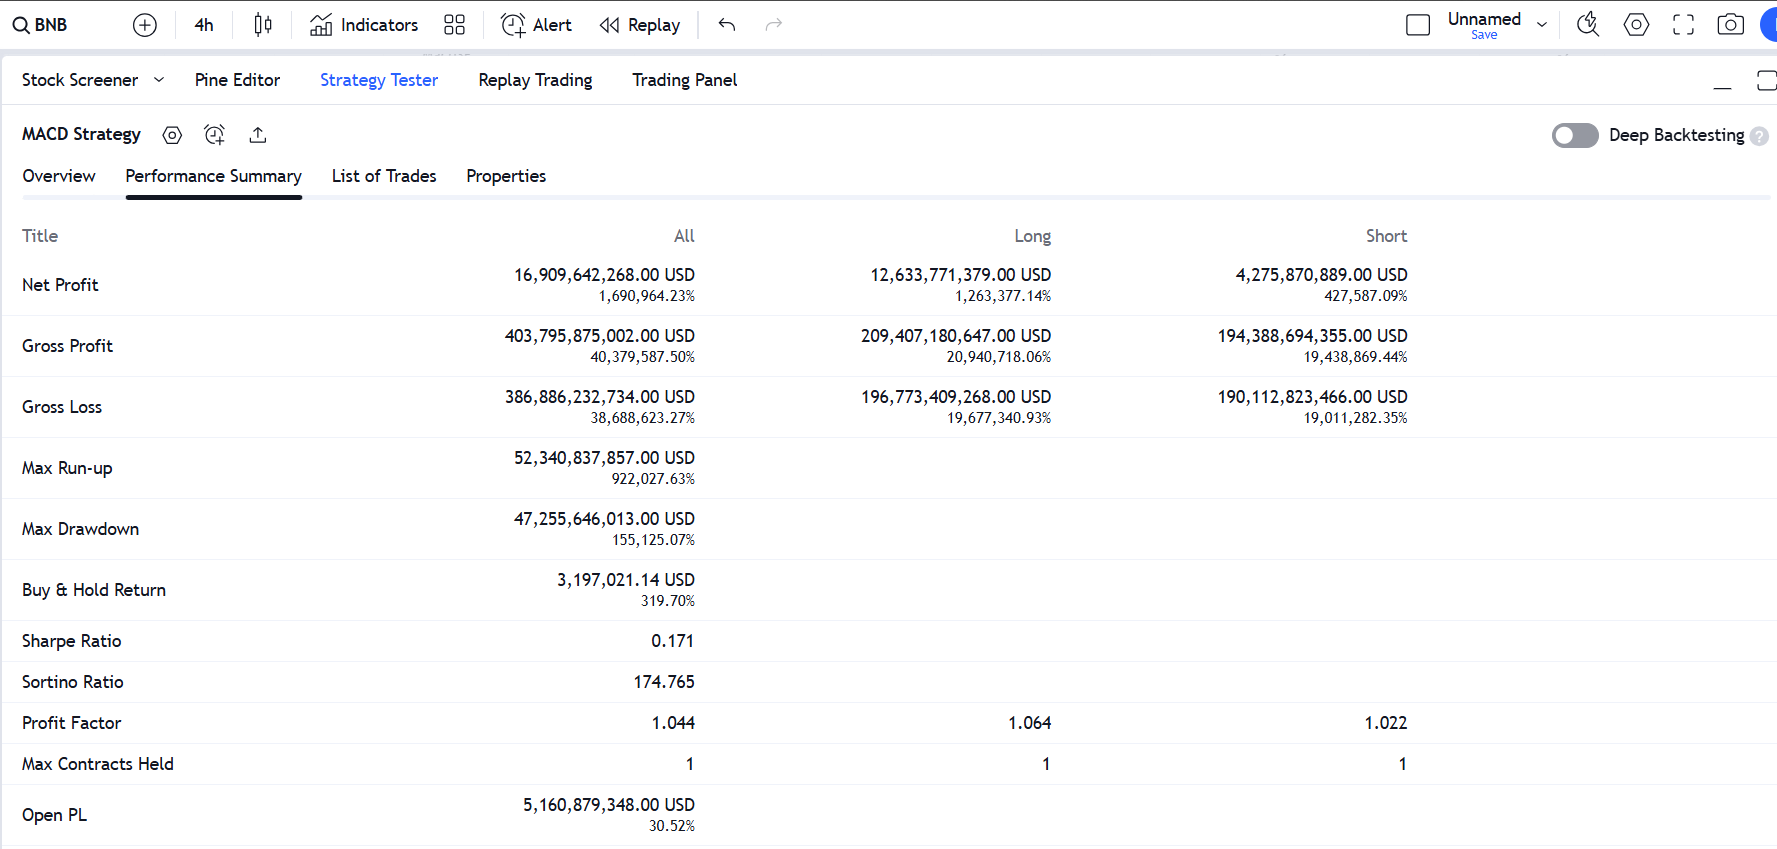
\includegraphics[scale=0.15]{pic_14.png}\label{p14}}
\end{figure}
\newpage
تست استراتژی برروی رمزارز \lr{DOGE}
\begin{figure}[H]
	\centering
	\subfloat[
	عملکرد ترکیب استراتژی‌های \lr{EMA} و \lr{RSI} برروی رمزارز \lr{DOGE}
	]{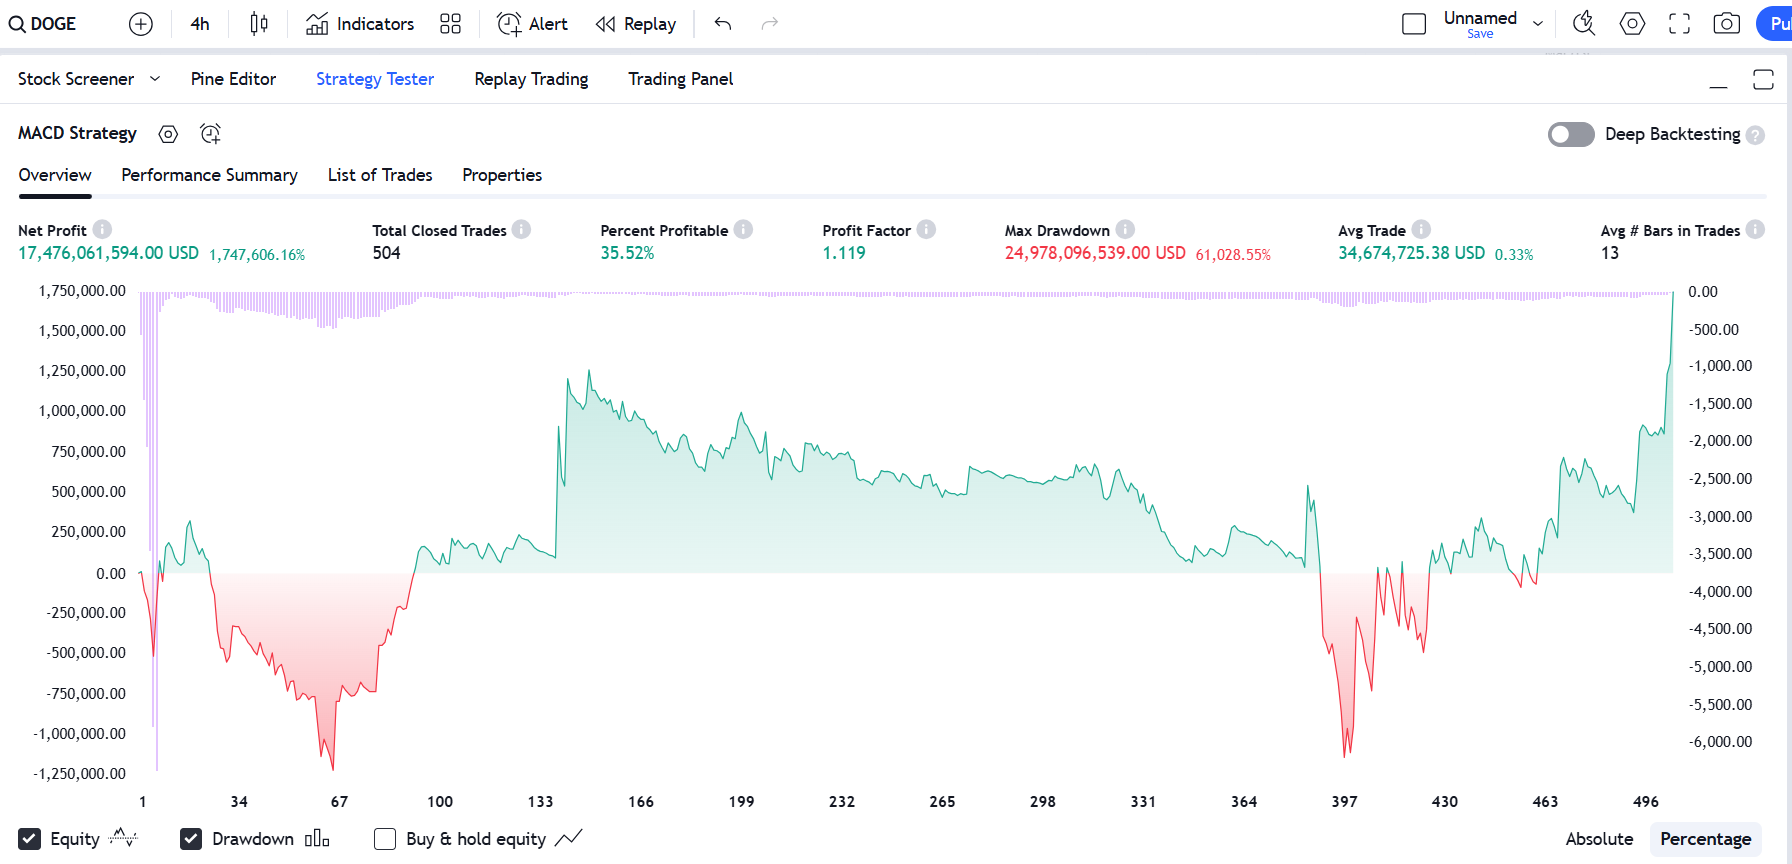
\includegraphics[scale=0.15]{pic_15.png}\label{p15}}
	\quad \quad
	\subfloat[
	سود و زیان ترکیب استراتژی \lr{EMA} و \lr{RSI}
	]{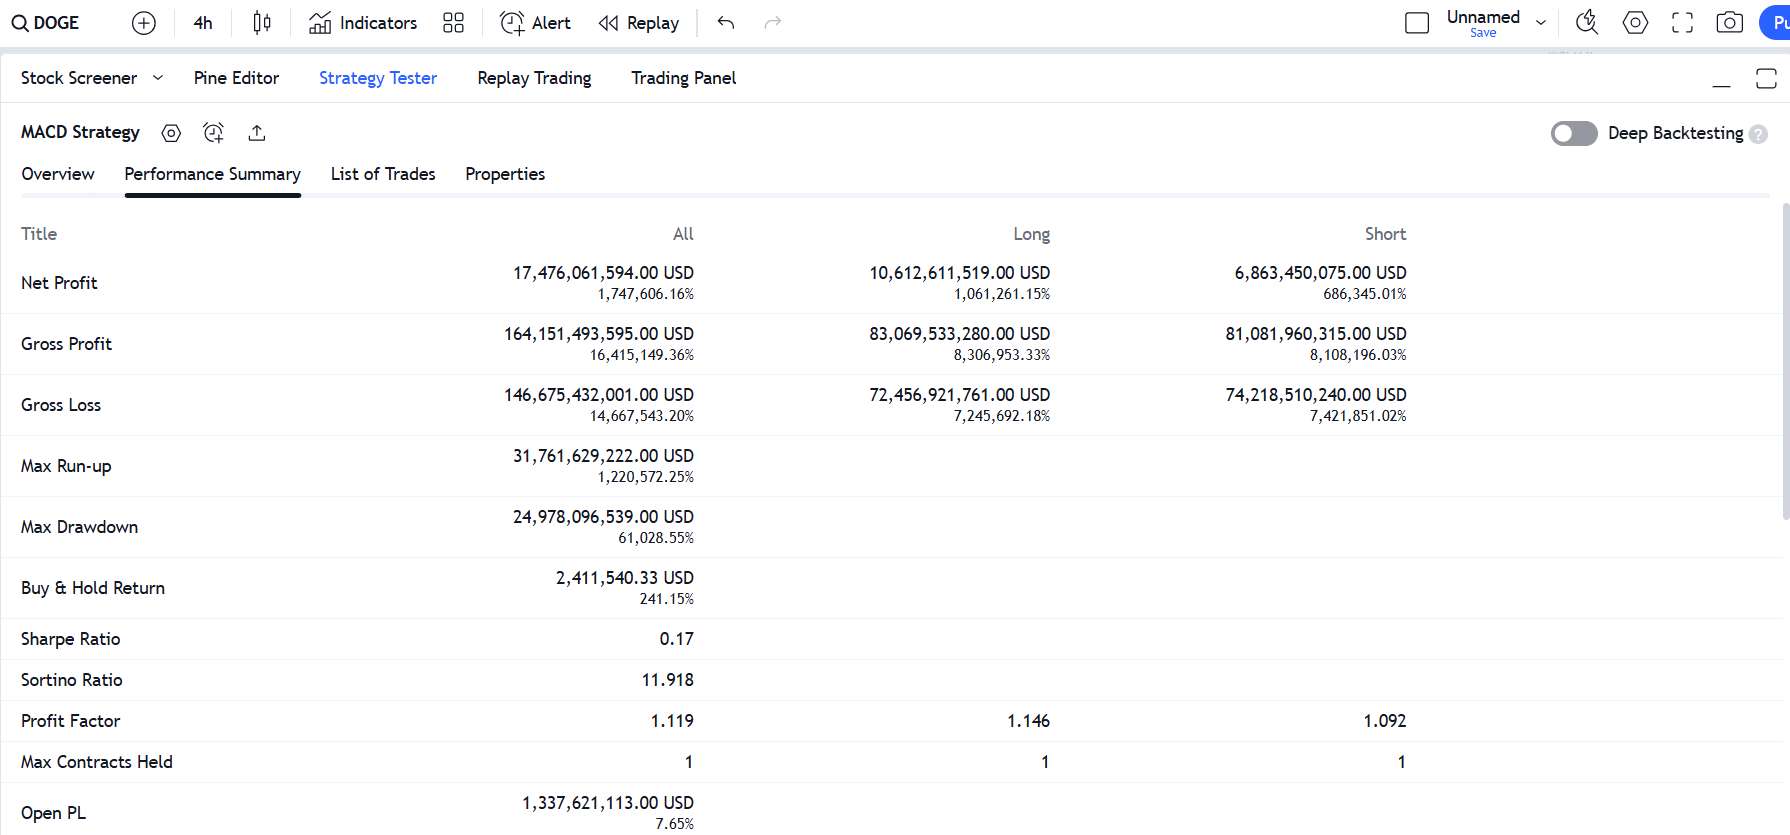
\includegraphics[scale=0.15]{pic_16.png}\label{p16}}
\end{figure}
تست استراتژی برروی رمزارز \lr{ُTONCOIN}
\begin{figure}[H]
	\centering
	\subfloat[
	عملکرد ترکیب استراتژی‌های \lr{EMA} و \lr{RSI} برروی رمزارز \lr{ُTONCOIN}
	]{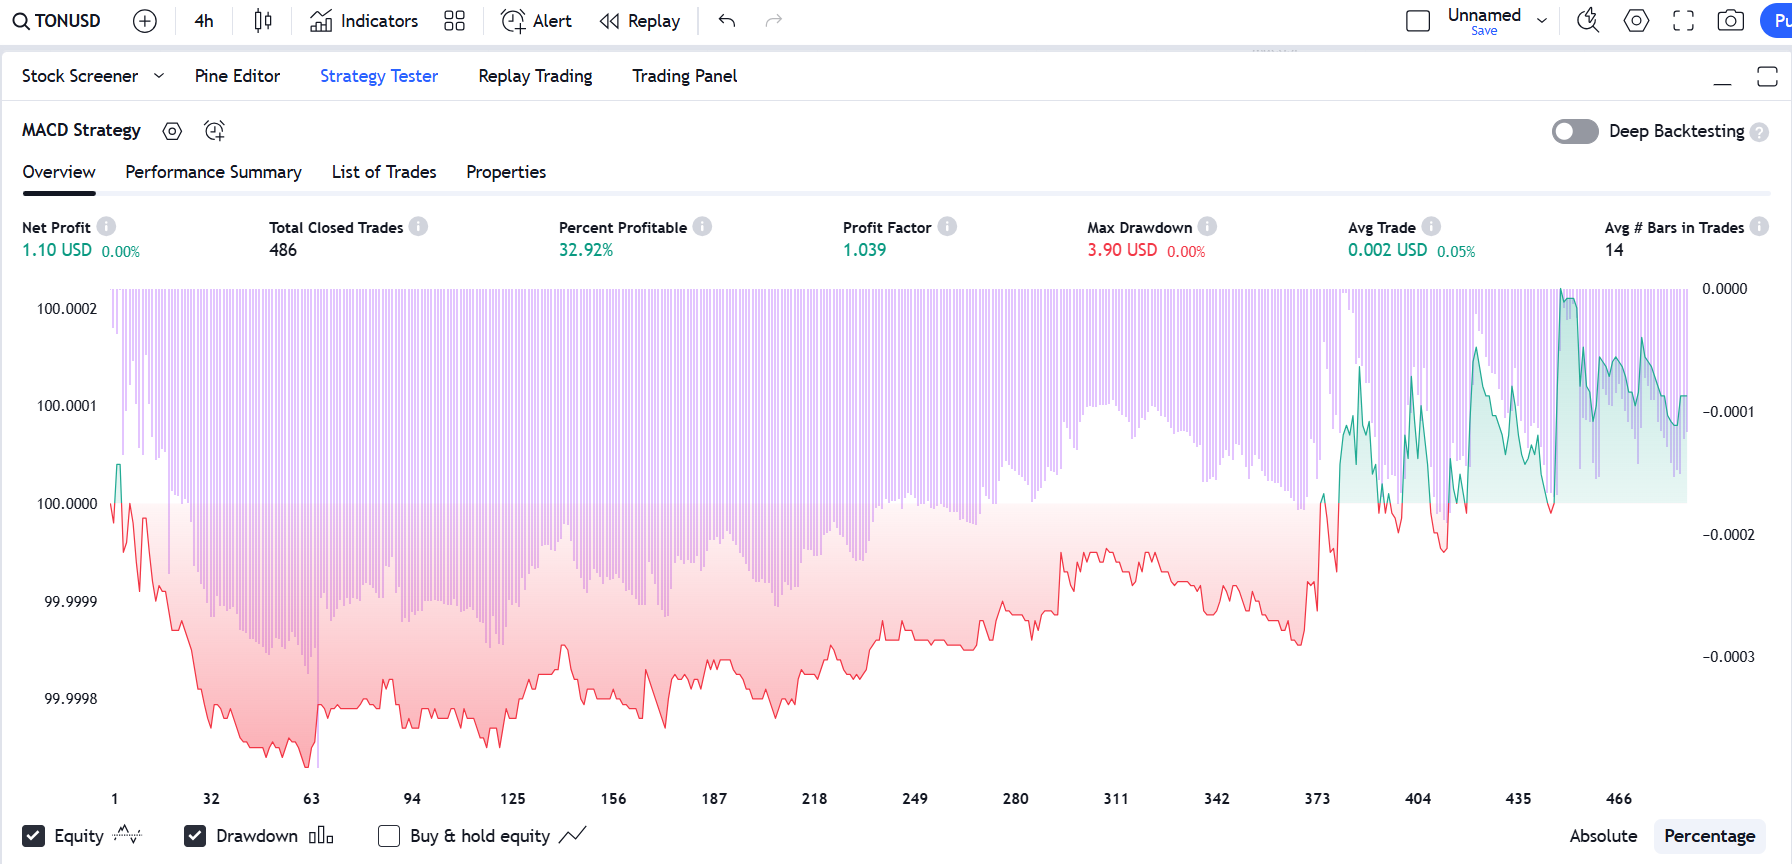
\includegraphics[scale=0.15]{pic_17.png}\label{p17}}
	\quad \quad
	\subfloat[
	سود و زیان ترکیب استراتژی \lr{EMA} و \lr{RSI}
	]{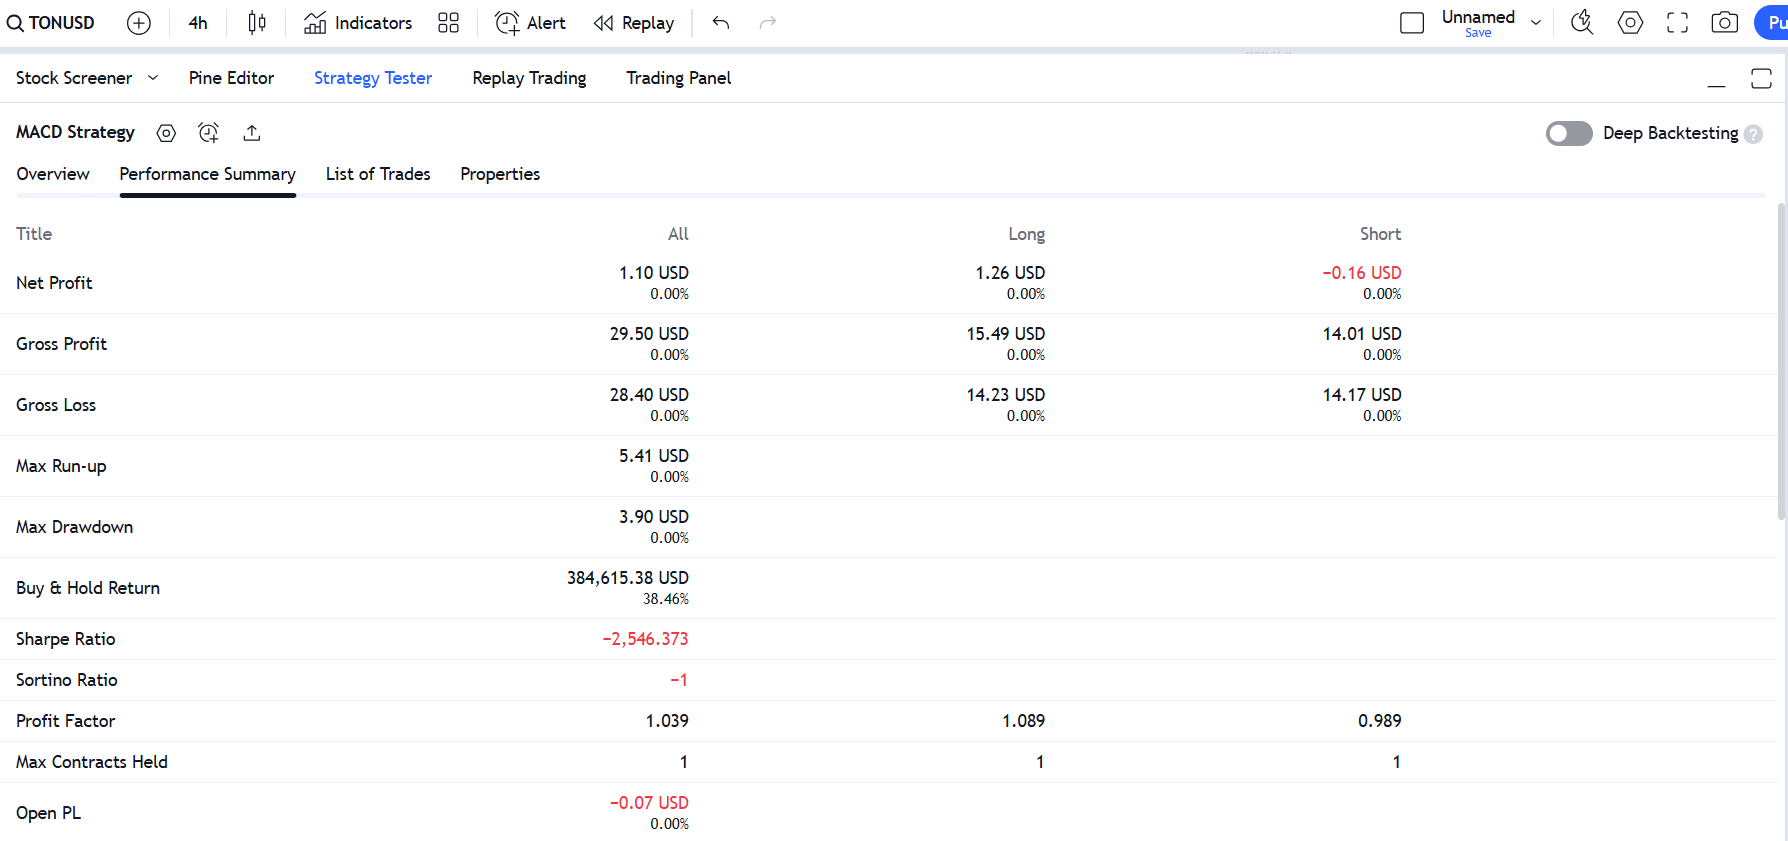
\includegraphics[scale=0.15]{pic_18.png}\label{p18}}
\end{figure}
تست استراتژی برروی رمزارز \lr{ADAUSD}
\begin{figure}[H]
	\centering
	\subfloat[
	عملکرد ترکیب استراتژی‌های \lr{EMA} و \lr{RSI} برروی رمزارز \lr{ADAUSD}
	]{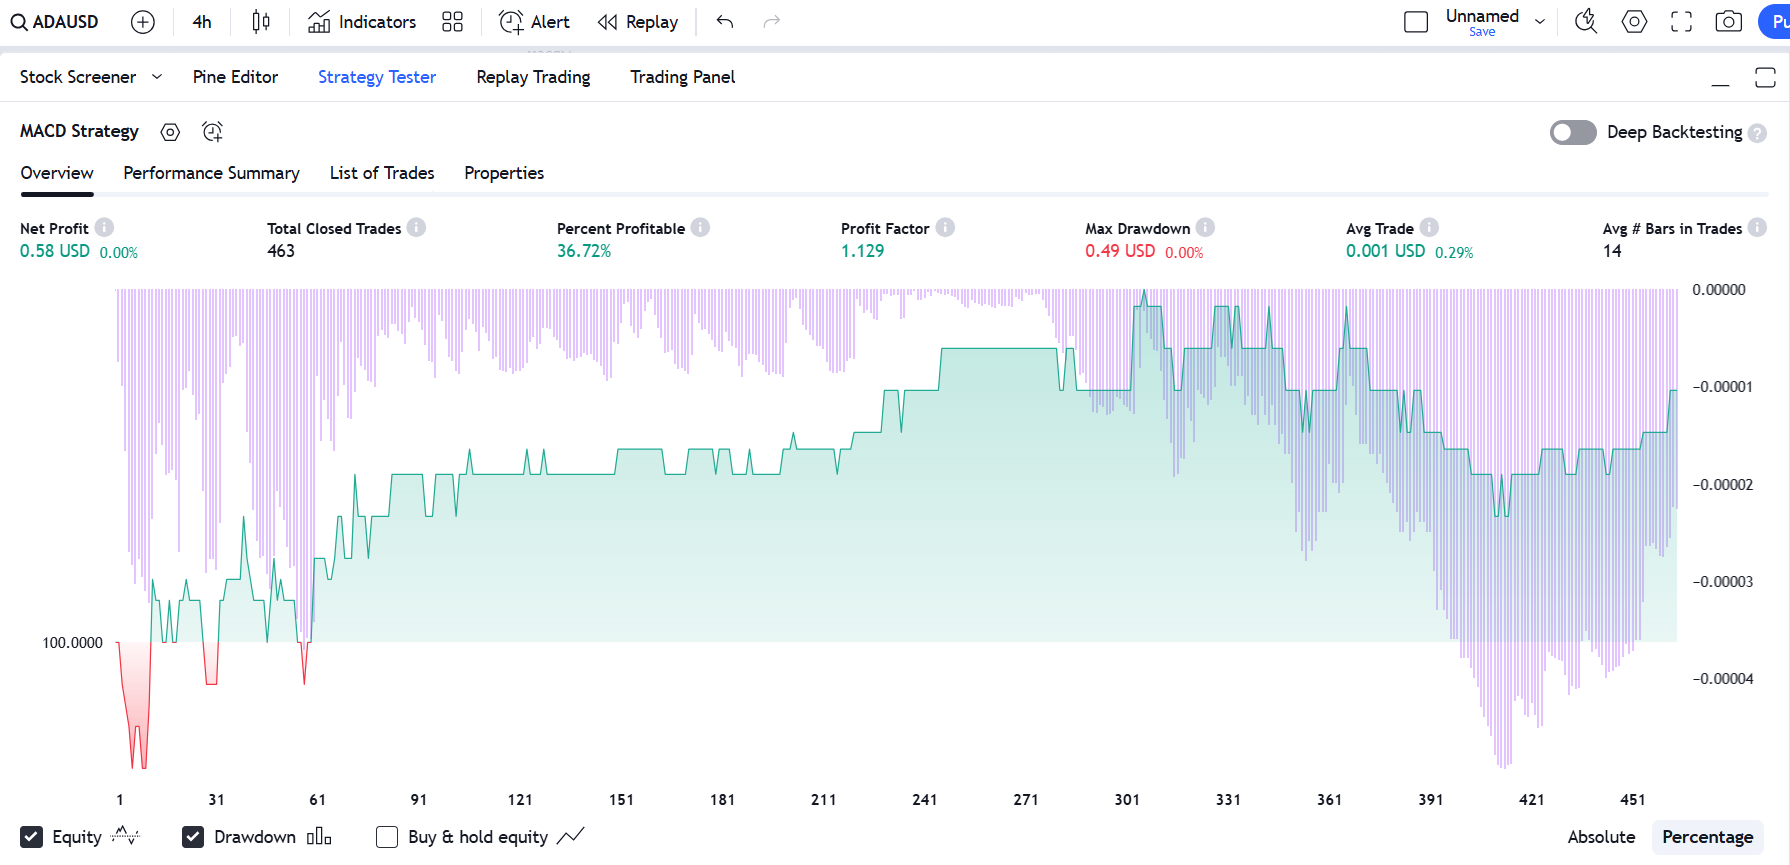
\includegraphics[scale=0.15]{pic_19.png}\label{p19}}
	\quad \quad
	\subfloat[
	سود و زیان ترکیب استراتژی \lr{EMA} و \lr{RSI}
	]{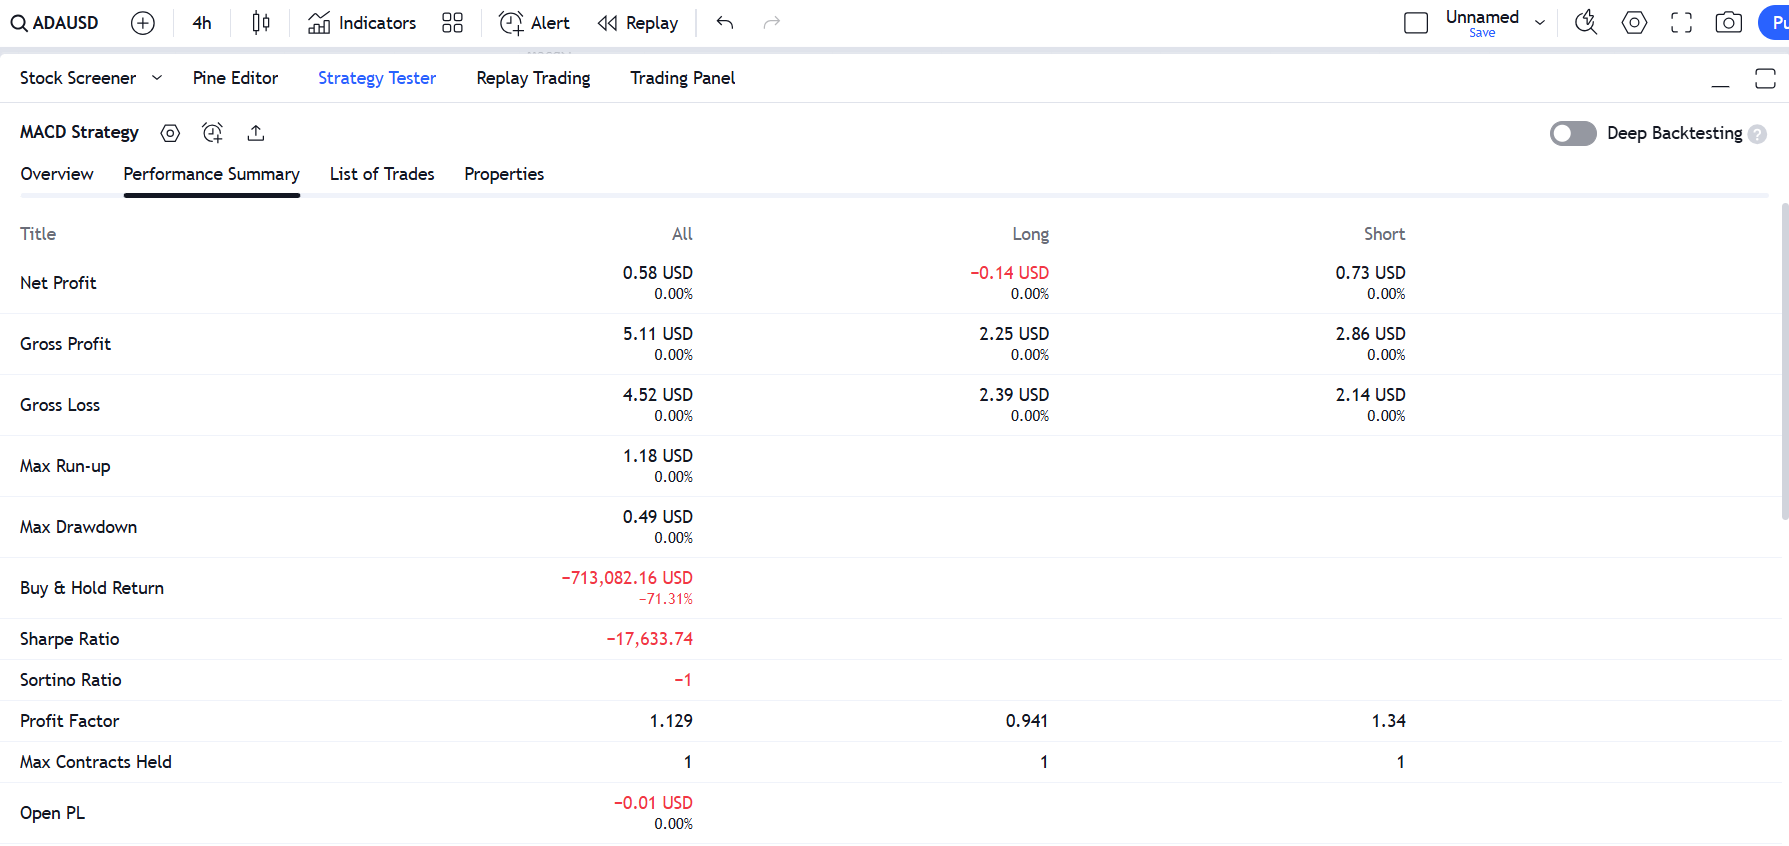
\includegraphics[scale=0.15]{pic_20.png}\label{p20}}
\end{figure}
لازم به ذکر است که استراتژی برروی بازه‌های دوساله از رمزارزها تست شده است.
\section{Sharpe Ratio}
در تمام موارد زیر، وجود یک بازه مثبت حداقل سه ماهه برای رمزارزها مشخص است. برای ترسیم \lr{Sharpe Ratio} از اندیکاتور \lr{"Sharpe and Sortino Ratios"}متعلق به سایت \lr{TradingView}استفاده شده است و تنها \lr{Sharpe Ratio} نمایش داده شده است.
\begin{figure}[H]
	\centering
	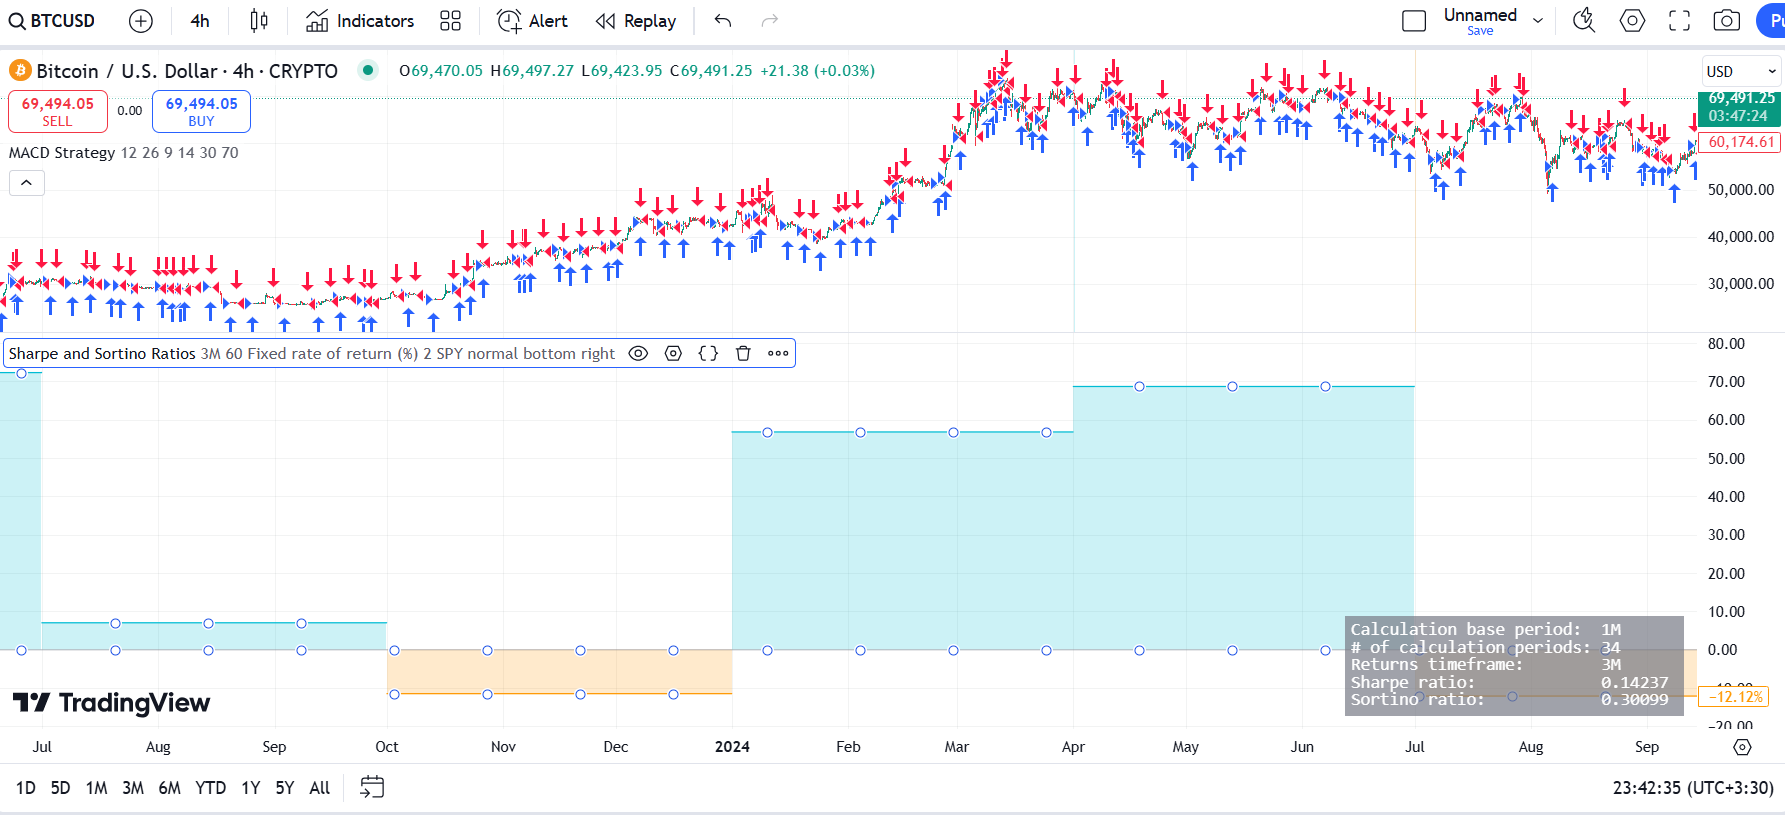
\includegraphics[scale=0.3]{pic_21.png}
	\caption{\lr{Sharpe Ratio for BTC}}
\end{figure}
\begin{figure}[H]
	\centering
	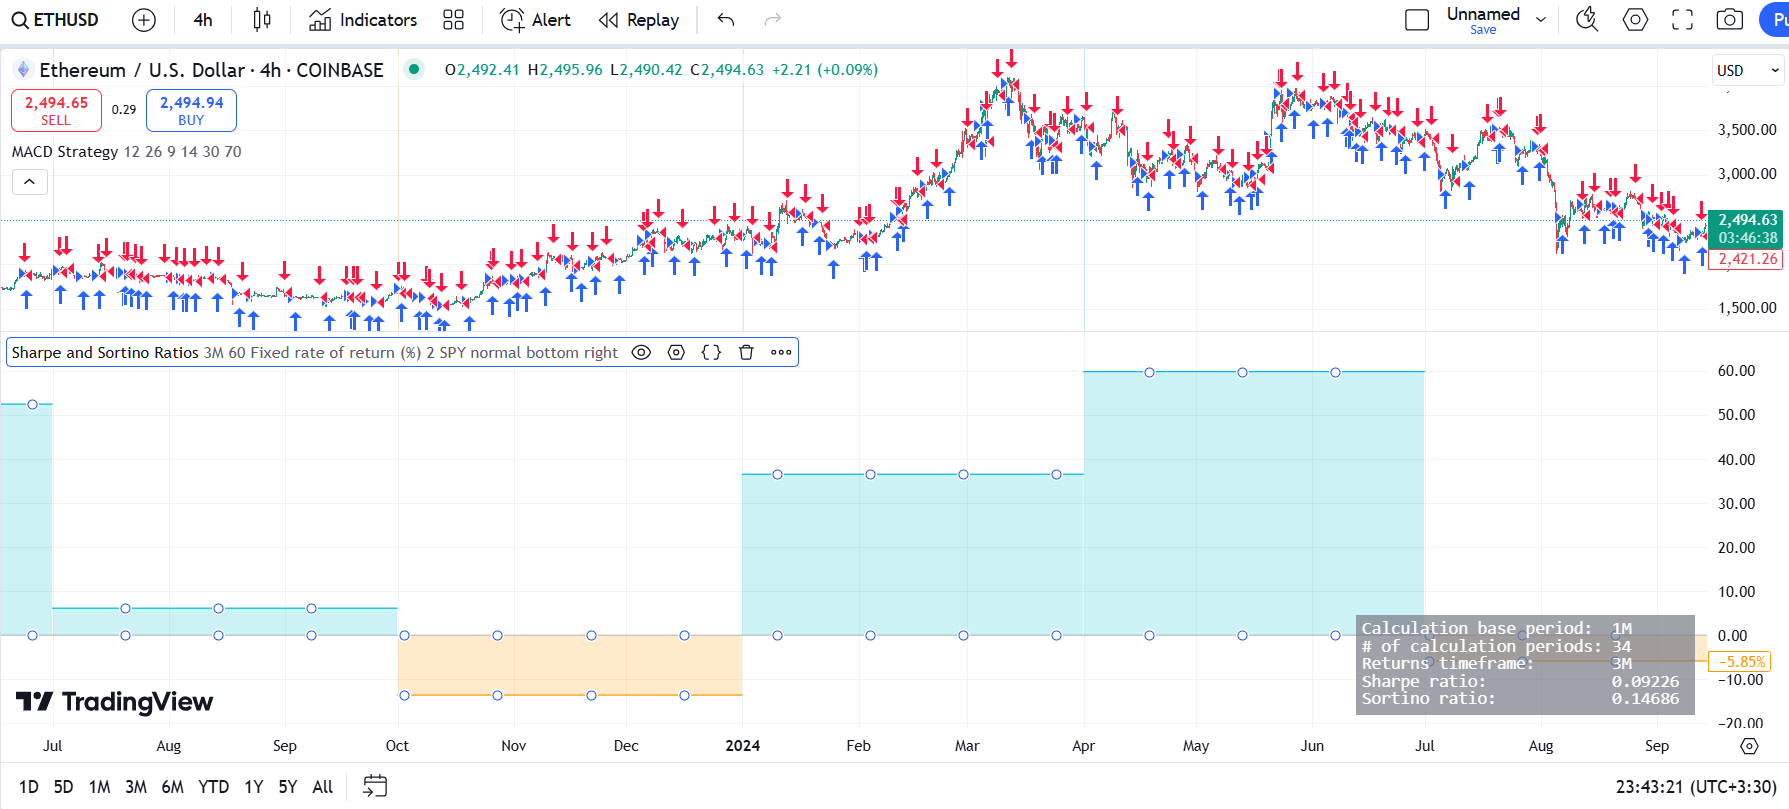
\includegraphics[scale=0.3]{pic_22.png}
	
	\caption{\lr{Sharpe Ratio for ETH}}
\end{figure}
\begin{figure}[H]
	\centering
	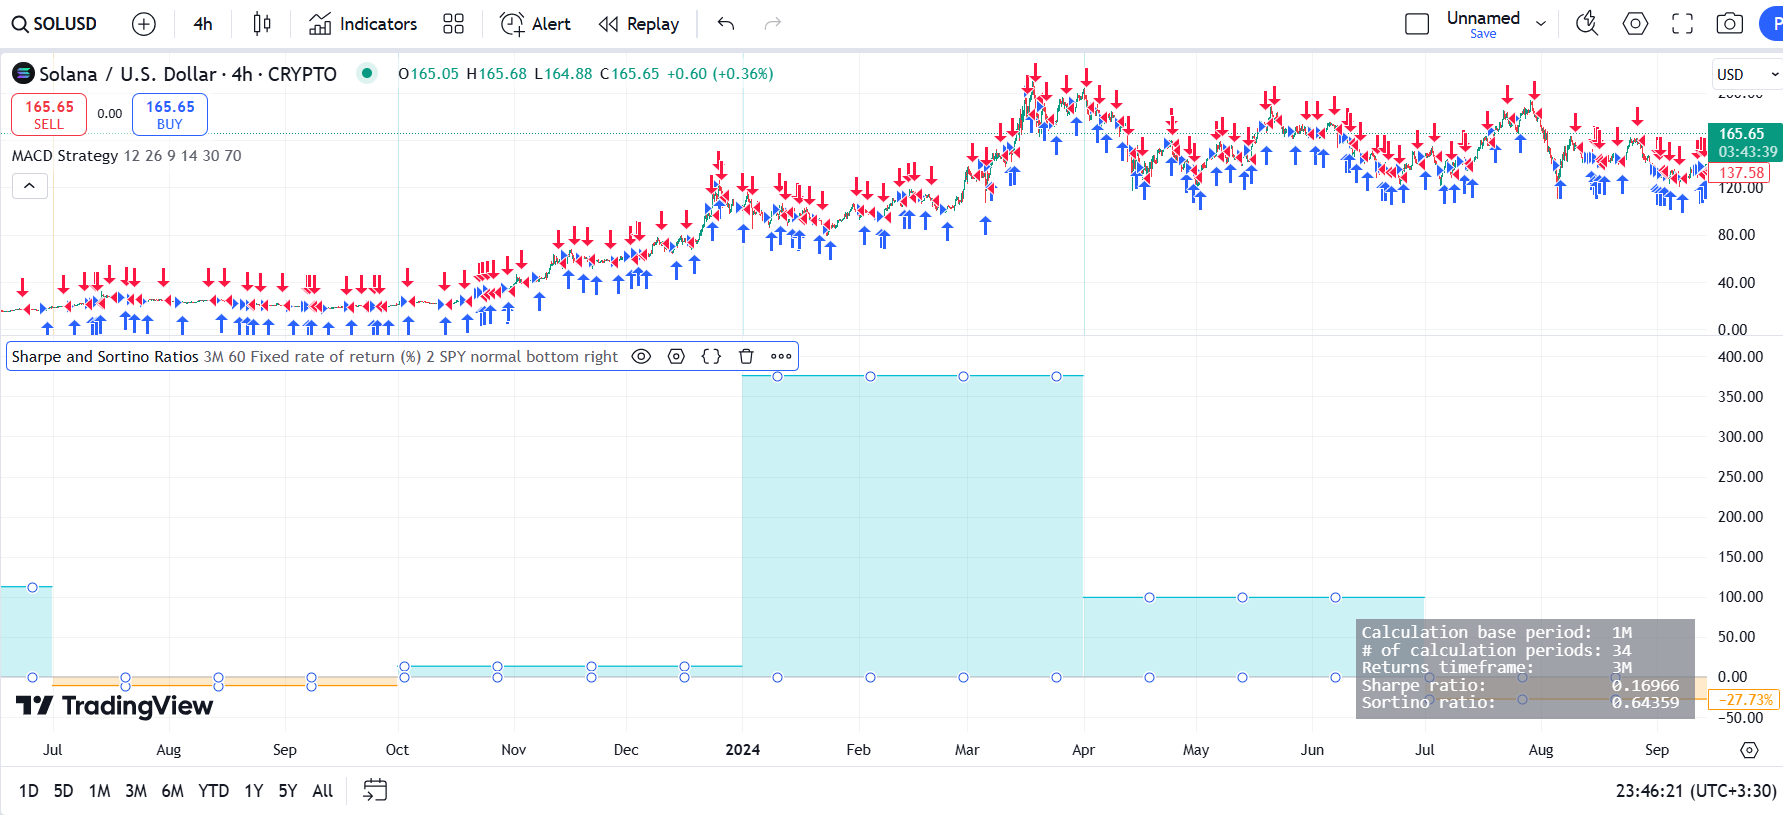
\includegraphics[scale=0.3]{pic_23.png}
	\caption{\lr{Sharpe Ratio for SOLANA}}
\end{figure}
\begin{figure}[H]
	\centering
	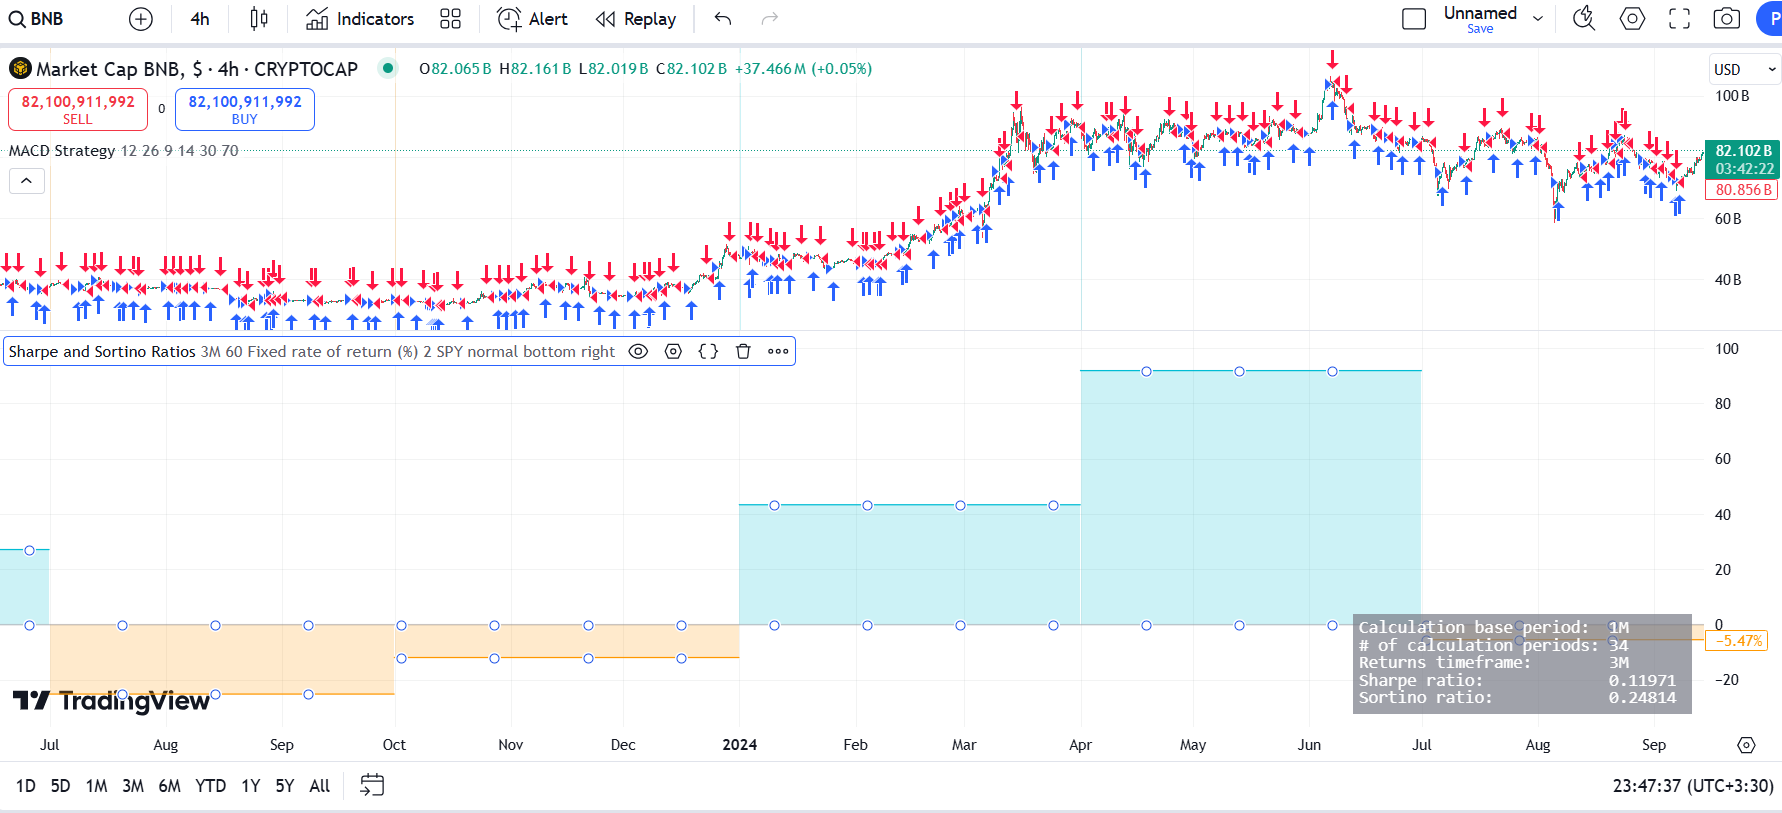
\includegraphics[scale=0.3]{pic_24.png}
	\caption{\lr{Sharpe Ratio for BNB}}
\end{figure}
\begin{figure}[H]
	\centering
	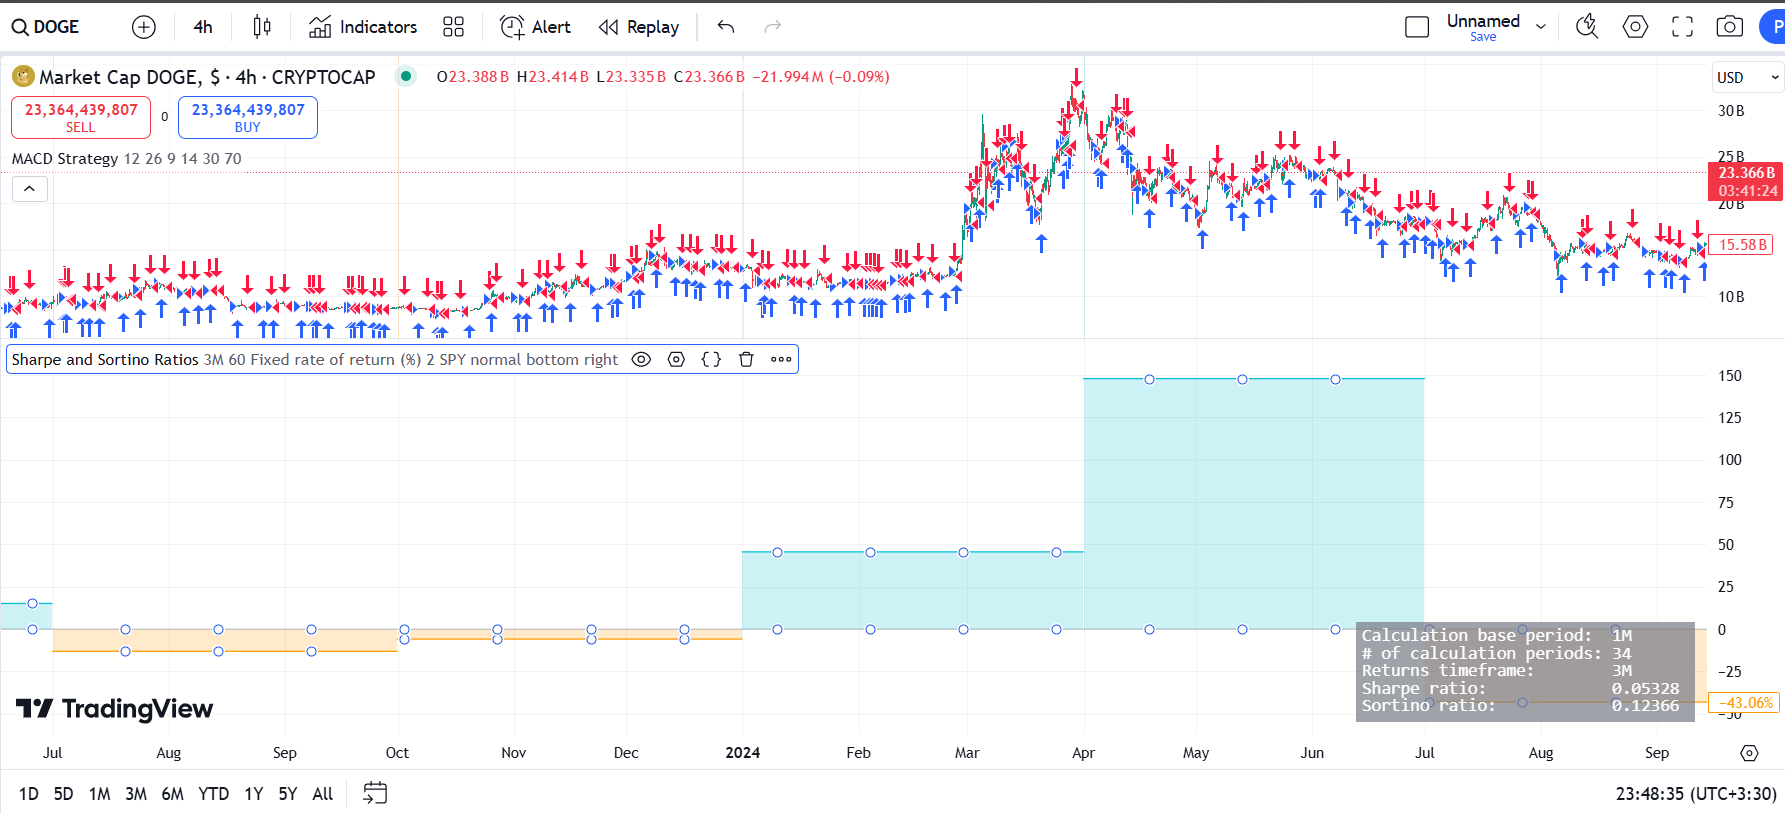
\includegraphics[scale=0.3]{pic_25.png}
	\caption{\lr{Sharpe Ratio for DOGE}}
\end{figure}
\begin{figure}[H]
	\centering
	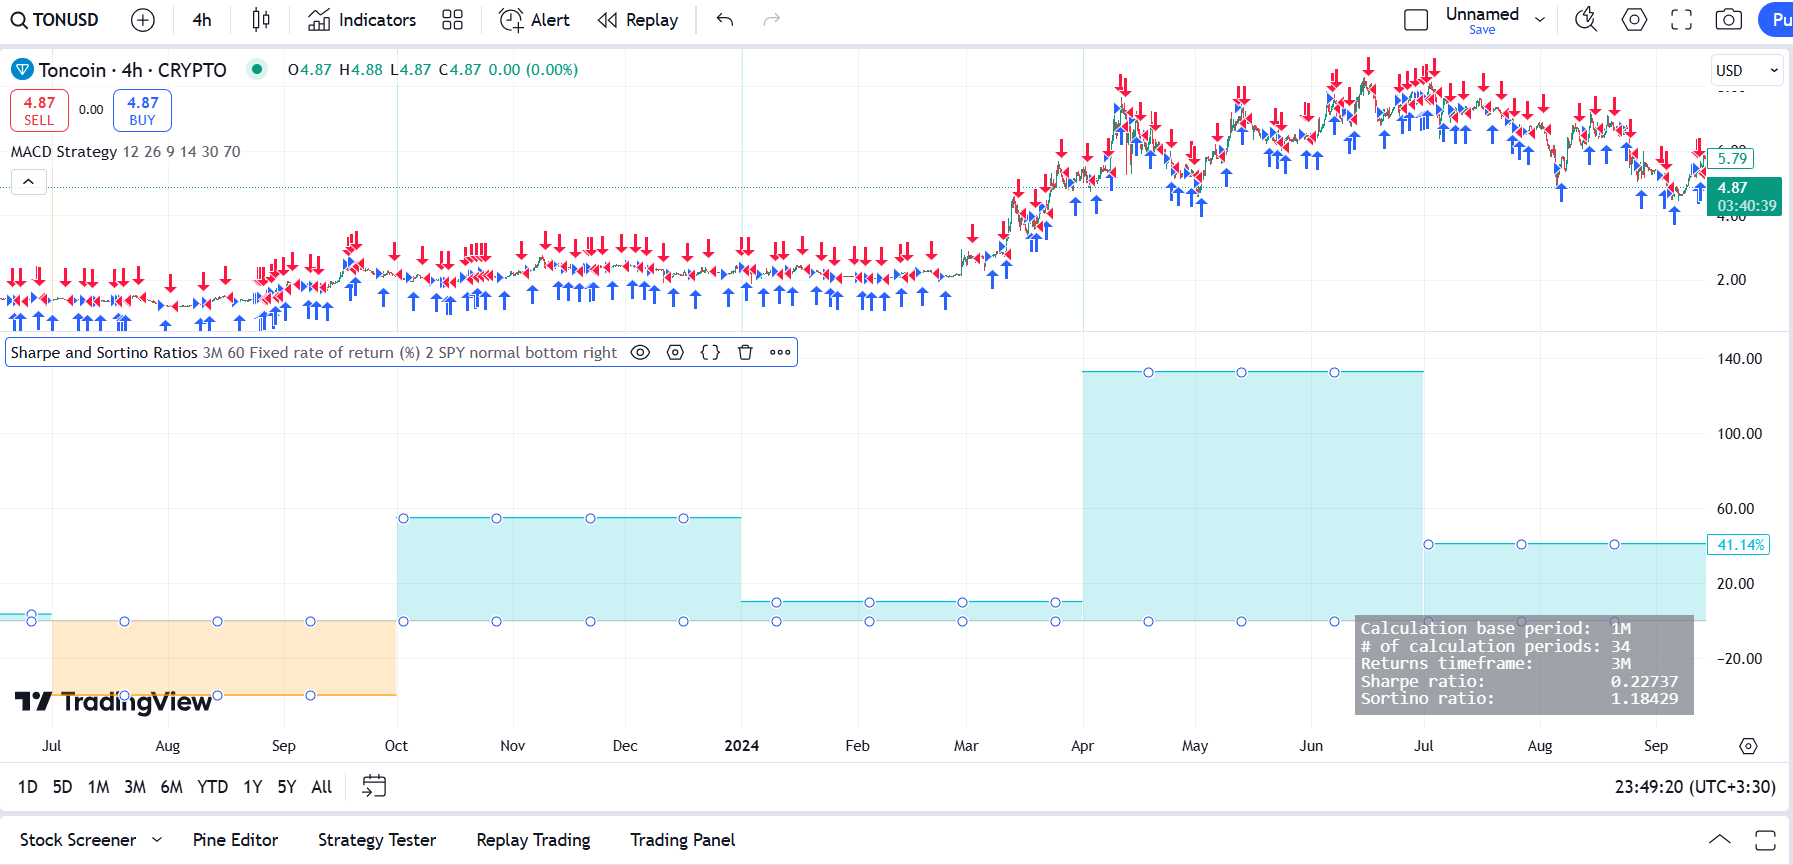
\includegraphics[scale=0.3]{pic_26.png}
	\caption{\lr{Sharpe Ratio for TONCOIN}}
\end{figure}
\begin{figure}[H]
	\centering
	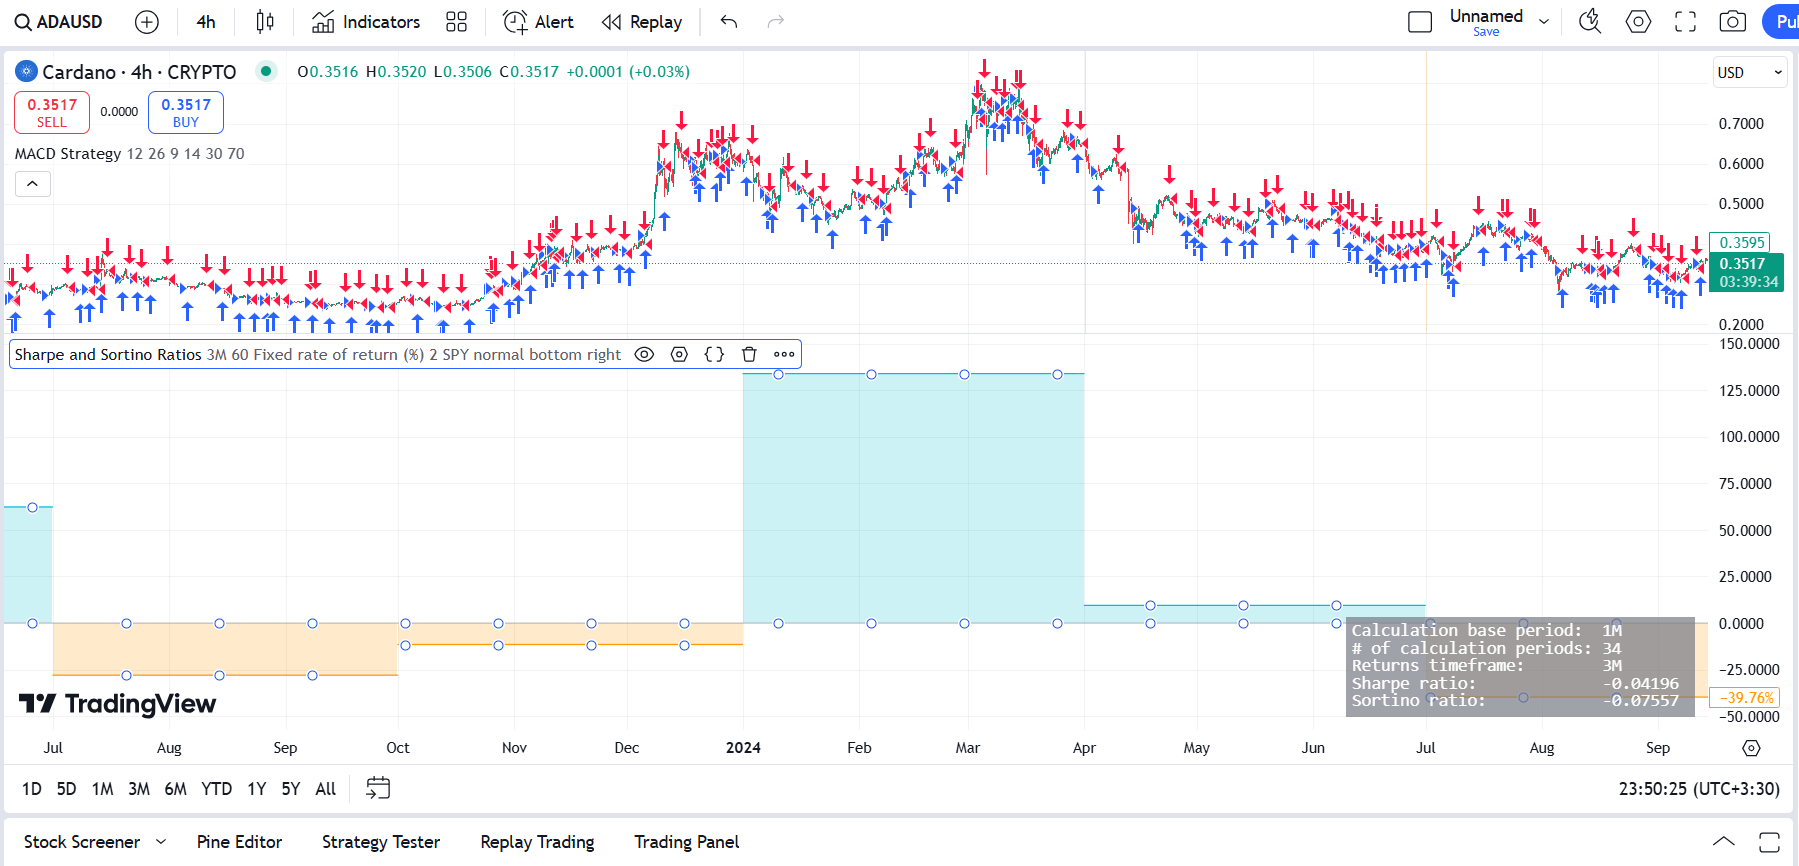
\includegraphics[scale=0.3]{pic_27.png}
	\caption{\lr{Sharpe Ratio for ADAUSD}}
\end{figure}
\end{document}